


<!DOCTYPE html>
<html lang="en" class="">
  <head prefix="og: http://ogp.me/ns# fb: http://ogp.me/ns/fb# object: http://ogp.me/ns/object# article: http://ogp.me/ns/article# profile: http://ogp.me/ns/profile#">
    <meta charset='utf-8'>
    <meta http-equiv="X-UA-Compatible" content="IE=edge">
    <meta http-equiv="Content-Language" content="en">
    <meta name="viewport" content="width=1020">
    
    
    <title>MorganLevy_Evolang11/MorganLevy_evolang11-draft3.tex at 892b9b465361251af2a39631a189adfe3c1453bc · dumble/MorganLevy_Evolang11</title>
    <link rel="search" type="application/opensearchdescription+xml" href="/opensearch.xml" title="GitHub">
    <link rel="fluid-icon" href="https://github.com/fluidicon.png" title="GitHub">
    <link rel="apple-touch-icon" sizes="57x57" href="/apple-touch-icon-114.png">
    <link rel="apple-touch-icon" sizes="114x114" href="/apple-touch-icon-114.png">
    <link rel="apple-touch-icon" sizes="72x72" href="/apple-touch-icon-144.png">
    <link rel="apple-touch-icon" sizes="144x144" href="/apple-touch-icon-144.png">
    <meta property="fb:app_id" content="1401488693436528">

      <meta content="@github" name="twitter:site" /><meta content="summary" name="twitter:card" /><meta content="dumble/MorganLevy_Evolang11" name="twitter:title" /><meta content="Contribute to MorganLevy_Evolang11 development by creating an account on GitHub." name="twitter:description" /><meta content="https://avatars3.githubusercontent.com/u/7561787?v=3&amp;s=400" name="twitter:image:src" />
      <meta content="GitHub" property="og:site_name" /><meta content="object" property="og:type" /><meta content="https://avatars3.githubusercontent.com/u/7561787?v=3&amp;s=400" property="og:image" /><meta content="dumble/MorganLevy_Evolang11" property="og:title" /><meta content="https://github.com/dumble/MorganLevy_Evolang11" property="og:url" /><meta content="Contribute to MorganLevy_Evolang11 development by creating an account on GitHub." property="og:description" />
      <meta name="browser-stats-url" content="https://api.github.com/_private/browser/stats">
    <meta name="browser-errors-url" content="https://api.github.com/_private/browser/errors">
    <link rel="assets" href="https://assets-cdn.github.com/">
    <link rel="web-socket" href="wss://live.github.com/_sockets/NzU2MTc4NzpmOTNjZmZjZDFlODFhMjBjZGZmNzM3MDViN2QyY2I2ZToxM2Y3ZmU1NDI5ODQ5YWQ2YTZjM2JiMDUwYzlkYTA2ZDVjMmUzOTU5OTFkMTUzOGMxNjhjMzYyOTc3ZTI5MTlj--0c616bed24ad71cee1d7f6f676e1e2bfd65c2f3a">
    <meta name="pjax-timeout" content="1000">
    <link rel="sudo-modal" href="/sessions/sudo_modal">

    <meta name="msapplication-TileImage" content="/windows-tile.png">
    <meta name="msapplication-TileColor" content="#ffffff">
    <meta name="selected-link" value="repo_source" data-pjax-transient>

    <meta name="google-site-verification" content="KT5gs8h0wvaagLKAVWq8bbeNwnZZK1r1XQysX3xurLU">
        <meta name="google-analytics" content="UA-3769691-2">

    <meta content="collector.githubapp.com" name="octolytics-host" /><meta content="collector-cdn.github.com" name="octolytics-script-host" /><meta content="github" name="octolytics-app-id" /><meta content="4408A649:3FB8:2683FC4:55FCDFD5" name="octolytics-dimension-request_id" /><meta content="7561787" name="octolytics-actor-id" /><meta content="dumble" name="octolytics-actor-login" /><meta content="725596323c4fe8a540c31ae4badda0cc37d30c742cdf36cf0b9cbec4b42be34d" name="octolytics-actor-hash" />
    
    <meta content="Rails, view, blob#show" data-pjax-transient="true" name="analytics-event" />
    <meta class="js-ga-set" name="dimension1" content="Logged In">
      <meta class="js-ga-set" name="dimension4" content="Current repo nav">
    <meta name="is-dotcom" content="true">
        <meta name="hostname" content="github.com">
    <meta name="user-login" content="dumble">

      <link rel="mask-icon" href="https://assets-cdn.github.com/pinned-octocat.svg" color="#4078c0">
      <link rel="icon" type="image/x-icon" href="https://assets-cdn.github.com/favicon.ico">

    <!-- </textarea> --><!-- '"` --><meta content="authenticity_token" name="csrf-param" />
<meta content="HeqszsNySfGQHpvYsGzT0fn7/ALYfjnRRb2uN+l2Lwj2XqvPTfuHHuwNrZdHhwfOIe+HnVWsojaPPkFpiCJGlA==" name="csrf-token" />
    <meta content="ca393cf9bee5d90663991eaa57d00149899515d1" name="form-nonce" />

    <link crossorigin="anonymous" href="https://assets-cdn.github.com/assets/github-aef3088517c60128e10c5cce8d392985504018745a58a13691f1a278951852bb.css" media="all" rel="stylesheet" />
    <link crossorigin="anonymous" href="https://assets-cdn.github.com/assets/github2-eba1f472eb1c7c893e4310c05138905845443f7f2469812a9bd2ba71aa488cc5.css" media="all" rel="stylesheet" />
    
    


    <meta http-equiv="x-pjax-version" content="87dbf4dad0b70976ed64b3bf4976701e">

      
  <meta name="description" content="Contribute to MorganLevy_Evolang11 development by creating an account on GitHub.">
  <meta name="go-import" content="github.com/dumble/MorganLevy_Evolang11 git https://github.com/dumble/MorganLevy_Evolang11.git">

  <meta content="7561787" name="octolytics-dimension-user_id" /><meta content="dumble" name="octolytics-dimension-user_login" /><meta content="42686571" name="octolytics-dimension-repository_id" /><meta content="dumble/MorganLevy_Evolang11" name="octolytics-dimension-repository_nwo" /><meta content="true" name="octolytics-dimension-repository_public" /><meta content="false" name="octolytics-dimension-repository_is_fork" /><meta content="42686571" name="octolytics-dimension-repository_network_root_id" /><meta content="dumble/MorganLevy_Evolang11" name="octolytics-dimension-repository_network_root_nwo" />
  <link href="https://github.com/dumble/MorganLevy_Evolang11/commits/892b9b465361251af2a39631a189adfe3c1453bc.atom" rel="alternate" title="Recent Commits to MorganLevy_Evolang11:892b9b465361251af2a39631a189adfe3c1453bc" type="application/atom+xml">

  </head>


  <body class="logged_in  env-production macintosh vis-public page-blob">
    <a href="#start-of-content" tabindex="1" class="accessibility-aid js-skip-to-content">Skip to content</a>

    
    
    



      <div class="header header-logged-in true" role="banner">
  <div class="container clearfix">

    <a class="header-logo-invertocat" href="https://github.com/" data-hotkey="g d" aria-label="Homepage" data-ga-click="Header, go to dashboard, icon:logo">
  <span class="mega-octicon octicon-mark-github"></span>
</a>


      <div class="site-search repo-scope js-site-search" role="search">
          <!-- </textarea> --><!-- '"` --><form accept-charset="UTF-8" action="/dumble/MorganLevy_Evolang11/search" class="js-site-search-form" data-global-search-url="/search" data-repo-search-url="/dumble/MorganLevy_Evolang11/search" method="get"><div style="margin:0;padding:0;display:inline"><input name="utf8" type="hidden" value="&#x2713;" /></div>
  <label class="js-chromeless-input-container form-control">
    <div class="scope-badge">This repository</div>
    <input type="text"
      class="js-site-search-focus js-site-search-field is-clearable chromeless-input"
      data-hotkey="s"
      name="q"
      placeholder="Search"
      aria-label="Search this repository"
      data-global-scope-placeholder="Search GitHub"
      data-repo-scope-placeholder="Search"
      tabindex="1"
      autocapitalize="off">
  </label>
</form>
      </div>

      <ul class="header-nav left" role="navigation">
        <li class="header-nav-item">
          <a href="/pulls" class="js-selected-navigation-item header-nav-link" data-ga-click="Header, click, Nav menu - item:pulls context:user" data-hotkey="g p" data-selected-links="/pulls /pulls/assigned /pulls/mentioned /pulls">
            Pull requests
</a>        </li>
        <li class="header-nav-item">
          <a href="/issues" class="js-selected-navigation-item header-nav-link" data-ga-click="Header, click, Nav menu - item:issues context:user" data-hotkey="g i" data-selected-links="/issues /issues/assigned /issues/mentioned /issues">
            Issues
</a>        </li>
          <li class="header-nav-item">
            <a class="header-nav-link" href="https://gist.github.com/" data-ga-click="Header, go to gist, text:gist">Gist</a>
          </li>
      </ul>

    
<ul class="header-nav user-nav right" id="user-links">
  <li class="header-nav-item">
      <span class="js-socket-channel js-updatable-content"
        data-channel="notification-changed:dumble"
        data-url="/notifications/header">
      <a href="/notifications" aria-label="You have no unread notifications" class="header-nav-link notification-indicator tooltipped tooltipped-s" data-ga-click="Header, go to notifications, icon:read" data-hotkey="g n">
          <span class="mail-status all-read"></span>
          <span class="octicon octicon-bell"></span>
</a>  </span>

  </li>

  <li class="header-nav-item dropdown js-menu-container">
    <a class="header-nav-link tooltipped tooltipped-s js-menu-target" href="/new"
       aria-label="Create new…"
       data-ga-click="Header, create new, icon:add">
      <span class="octicon octicon-plus left"></span>
      <span class="dropdown-caret"></span>
    </a>

    <div class="dropdown-menu-content js-menu-content">
      <ul class="dropdown-menu dropdown-menu-sw">
        
<a class="dropdown-item" href="/new" data-ga-click="Header, create new repository">
  New repository
</a>


  <a class="dropdown-item" href="/organizations/new" data-ga-click="Header, create new organization">
    New organization
  </a>



  <div class="dropdown-divider"></div>
  <div class="dropdown-header">
    <span title="dumble/MorganLevy_Evolang11">This repository</span>
  </div>
    <a class="dropdown-item" href="/dumble/MorganLevy_Evolang11/issues/new" data-ga-click="Header, create new issue">
      New issue
    </a>
    <a class="dropdown-item" href="/dumble/MorganLevy_Evolang11/settings/collaboration" data-ga-click="Header, create new collaborator">
      New collaborator
    </a>

      </ul>
    </div>
  </li>

  <li class="header-nav-item dropdown js-menu-container">
    <a class="header-nav-link name tooltipped tooltipped-s js-menu-target" href="/dumble"
       aria-label="View profile and more"
       data-ga-click="Header, show menu, icon:avatar">
      <img alt="@dumble" class="avatar" height="20" src="https://avatars1.githubusercontent.com/u/7561787?v=3&amp;s=40" width="20" />
      <span class="dropdown-caret"></span>
    </a>

    <div class="dropdown-menu-content js-menu-content">
      <div class="dropdown-menu dropdown-menu-sw">
        <div class="dropdown-header header-nav-current-user css-truncate">
          Signed in as <strong class="css-truncate-target">dumble</strong>
        </div>
        <div class="dropdown-divider"></div>

        <a class="dropdown-item" href="/dumble" data-ga-click="Header, go to profile, text:your profile">
          Your profile
        </a>
        <a class="dropdown-item" href="/stars" data-ga-click="Header, go to starred repos, text:your stars">
          Your stars
        </a>
        <a class="dropdown-item" href="/explore" data-ga-click="Header, go to explore, text:explore">
          Explore
        </a>
        <a class="dropdown-item" href="https://help.github.com" data-ga-click="Header, go to help, text:help">
          Help
        </a>
        <div class="dropdown-divider"></div>

        <a class="dropdown-item" href="/settings/profile" data-ga-click="Header, go to settings, icon:settings">
          Settings
        </a>

        <!-- </textarea> --><!-- '"` --><form accept-charset="UTF-8" action="/logout" class="logout-form" data-form-nonce="ca393cf9bee5d90663991eaa57d00149899515d1" method="post"><div style="margin:0;padding:0;display:inline"><input name="utf8" type="hidden" value="&#x2713;" /><input name="authenticity_token" type="hidden" value="Rm4kSyN8jDABAUE6Flbf3ExPehG42AKWme560LPEp5zIRcIaJDAHLMME8I1iW01Lku0KI8TiRU+ITVS9nQrMwQ==" /></div>
          <button class="dropdown-item dropdown-signout" data-ga-click="Header, sign out, icon:logout">
            Sign out
          </button>
</form>      </div>
    </div>
  </li>
</ul>


    
  </div>
</div>

      

      


    <div id="start-of-content" class="accessibility-aid"></div>

    <div id="js-flash-container">
</div>


    <div role="main" class="main-content">
        <div itemscope itemtype="http://schema.org/WebPage">
    <div class="pagehead repohead instapaper_ignore readability-menu">

      <div class="container">

        <div class="clearfix">
          
<ul class="pagehead-actions">

  <li>
      <!-- </textarea> --><!-- '"` --><form accept-charset="UTF-8" action="/notifications/subscribe" class="js-social-container" data-autosubmit="true" data-form-nonce="ca393cf9bee5d90663991eaa57d00149899515d1" data-remote="true" method="post"><div style="margin:0;padding:0;display:inline"><input name="utf8" type="hidden" value="&#x2713;" /><input name="authenticity_token" type="hidden" value="6mzVCJcke9YG9HjjcNRPnCufcZWa7Fqv2siHoZF2JENKkhSdgrG1xL0GNkySIsdHmECQBlouWpmaybgCoFIvVQ==" /></div>    <input id="repository_id" name="repository_id" type="hidden" value="42686571" />

      <div class="select-menu js-menu-container js-select-menu">
        <a href="/dumble/MorganLevy_Evolang11/subscription"
          class="btn btn-sm btn-with-count select-menu-button js-menu-target" role="button" tabindex="0" aria-haspopup="true"
          data-ga-click="Repository, click Watch settings, action:blob#show">
          <span class="js-select-button">
            <span class="octicon octicon-eye"></span>
            Unwatch
          </span>
        </a>
        <a class="social-count js-social-count" href="/dumble/MorganLevy_Evolang11/watchers">
          2
        </a>

        <div class="select-menu-modal-holder">
          <div class="select-menu-modal subscription-menu-modal js-menu-content" aria-hidden="true">
            <div class="select-menu-header">
              <span class="select-menu-title">Notifications</span>
              <span class="octicon octicon-x js-menu-close" role="button" aria-label="Close"></span>
            </div>

            <div class="select-menu-list js-navigation-container" role="menu">

              <div class="select-menu-item js-navigation-item " role="menuitem" tabindex="0">
                <span class="select-menu-item-icon octicon octicon-check"></span>
                <div class="select-menu-item-text">
                  <input id="do_included" name="do" type="radio" value="included" />
                  <span class="select-menu-item-heading">Not watching</span>
                  <span class="description">Be notified when participating or @mentioned.</span>
                  <span class="js-select-button-text hidden-select-button-text">
                    <span class="octicon octicon-eye"></span>
                    Watch
                  </span>
                </div>
              </div>

              <div class="select-menu-item js-navigation-item selected" role="menuitem" tabindex="0">
                <span class="select-menu-item-icon octicon octicon octicon-check"></span>
                <div class="select-menu-item-text">
                  <input checked="checked" id="do_subscribed" name="do" type="radio" value="subscribed" />
                  <span class="select-menu-item-heading">Watching</span>
                  <span class="description">Be notified of all conversations.</span>
                  <span class="js-select-button-text hidden-select-button-text">
                    <span class="octicon octicon-eye"></span>
                    Unwatch
                  </span>
                </div>
              </div>

              <div class="select-menu-item js-navigation-item " role="menuitem" tabindex="0">
                <span class="select-menu-item-icon octicon octicon-check"></span>
                <div class="select-menu-item-text">
                  <input id="do_ignore" name="do" type="radio" value="ignore" />
                  <span class="select-menu-item-heading">Ignoring</span>
                  <span class="description">Never be notified.</span>
                  <span class="js-select-button-text hidden-select-button-text">
                    <span class="octicon octicon-mute"></span>
                    Stop ignoring
                  </span>
                </div>
              </div>

            </div>

          </div>
        </div>
      </div>
</form>
  </li>

  <li>
    
  <div class="js-toggler-container js-social-container starring-container ">

    <!-- </textarea> --><!-- '"` --><form accept-charset="UTF-8" action="/dumble/MorganLevy_Evolang11/unstar" class="js-toggler-form starred js-unstar-button" data-form-nonce="ca393cf9bee5d90663991eaa57d00149899515d1" data-remote="true" method="post"><div style="margin:0;padding:0;display:inline"><input name="utf8" type="hidden" value="&#x2713;" /><input name="authenticity_token" type="hidden" value="G3s9ZECg14zDlANndD7fberi3iEPAwKf51gjKNRb/Cg4VM0xMJ9CX9GubKhf25yOlZhGInpFEUksdiGzodqiow==" /></div>
      <button
        class="btn btn-sm btn-with-count js-toggler-target"
        aria-label="Unstar this repository" title="Unstar dumble/MorganLevy_Evolang11"
        data-ga-click="Repository, click unstar button, action:blob#show; text:Unstar">
        <span class="octicon octicon-star"></span>
        Unstar
      </button>
        <a class="social-count js-social-count" href="/dumble/MorganLevy_Evolang11/stargazers">
          0
        </a>
</form>
    <!-- </textarea> --><!-- '"` --><form accept-charset="UTF-8" action="/dumble/MorganLevy_Evolang11/star" class="js-toggler-form unstarred js-star-button" data-form-nonce="ca393cf9bee5d90663991eaa57d00149899515d1" data-remote="true" method="post"><div style="margin:0;padding:0;display:inline"><input name="utf8" type="hidden" value="&#x2713;" /><input name="authenticity_token" type="hidden" value="Ny0i8bUyLhSffO4jxEyFsrx3YiFfOa5GPwFRJgm1NPerxnynCjBaU+MbBIj+j6GLLPaubhQer7Erz15N8iFbYQ==" /></div>
      <button
        class="btn btn-sm btn-with-count js-toggler-target"
        aria-label="Star this repository" title="Star dumble/MorganLevy_Evolang11"
        data-ga-click="Repository, click star button, action:blob#show; text:Star">
        <span class="octicon octicon-star"></span>
        Star
      </button>
        <a class="social-count js-social-count" href="/dumble/MorganLevy_Evolang11/stargazers">
          0
        </a>
</form>  </div>

  </li>

  <li>
          <!-- </textarea> --><!-- '"` --><form accept-charset="UTF-8" action="/dumble/MorganLevy_Evolang11/fork" class="btn-with-count" data-form-nonce="ca393cf9bee5d90663991eaa57d00149899515d1" method="post"><div style="margin:0;padding:0;display:inline"><input name="utf8" type="hidden" value="&#x2713;" /><input name="authenticity_token" type="hidden" value="eLEMpwCmVO9D8XeDk+z66pBREj+IDP7HWSDg305yf/BpgRQ83FziTv9Hqnh5tbcBSAUNKmip44wIXieITYjPpg==" /></div>
            <button
                type="submit"
                class="btn btn-sm btn-with-count"
                data-ga-click="Repository, show fork modal, action:blob#show; text:Fork"
                title="Fork your own copy of dumble/MorganLevy_Evolang11 to your account"
                aria-label="Fork your own copy of dumble/MorganLevy_Evolang11 to your account">
              <span class="octicon octicon-repo-forked"></span>
              Fork
            </button>
</form>
    <a href="/dumble/MorganLevy_Evolang11/network" class="social-count">
      0
    </a>
  </li>
</ul>

          <h1 itemscope itemtype="http://data-vocabulary.org/Breadcrumb" class="entry-title public ">
  <span class="mega-octicon octicon-repo"></span>
  <span class="author"><a href="/dumble" class="url fn" itemprop="url" rel="author"><span itemprop="title">dumble</span></a></span><!--
--><span class="path-divider">/</span><!--
--><strong><a href="/dumble/MorganLevy_Evolang11" data-pjax="#js-repo-pjax-container">MorganLevy_Evolang11</a></strong>

  <span class="page-context-loader">
    <img alt="" height="16" src="https://assets-cdn.github.com/images/spinners/octocat-spinner-32.gif" width="16" />
  </span>

</h1>

        </div>
      </div>
    </div>

    <div class="container">
      <div class="repository-with-sidebar repo-container new-discussion-timeline ">
        <div class="repository-sidebar clearfix">
          
<nav class="sunken-menu repo-nav js-repo-nav js-sidenav-container-pjax js-octicon-loaders"
     role="navigation"
     data-pjax="#js-repo-pjax-container"
     data-issue-count-url="/dumble/MorganLevy_Evolang11/issues/counts">
  <ul class="sunken-menu-group">
    <li class="tooltipped tooltipped-w" aria-label="Code">
      <a href="/dumble/MorganLevy_Evolang11" aria-label="Code" aria-selected="true" class="js-selected-navigation-item selected sunken-menu-item" data-hotkey="g c" data-selected-links="repo_source repo_downloads repo_commits repo_releases repo_tags repo_branches /dumble/MorganLevy_Evolang11">
        <span class="octicon octicon-code"></span> <span class="full-word">Code</span>
        <img alt="" class="mini-loader" height="16" src="https://assets-cdn.github.com/images/spinners/octocat-spinner-32.gif" width="16" />
</a>    </li>

      <li class="tooltipped tooltipped-w" aria-label="Issues">
        <a href="/dumble/MorganLevy_Evolang11/issues" aria-label="Issues" class="js-selected-navigation-item sunken-menu-item" data-hotkey="g i" data-selected-links="repo_issues repo_labels repo_milestones /dumble/MorganLevy_Evolang11/issues">
          <span class="octicon octicon-issue-opened"></span> <span class="full-word">Issues</span>
          <span class="js-issue-replace-counter"></span>
          <img alt="" class="mini-loader" height="16" src="https://assets-cdn.github.com/images/spinners/octocat-spinner-32.gif" width="16" />
</a>      </li>

    <li class="tooltipped tooltipped-w" aria-label="Pull requests">
      <a href="/dumble/MorganLevy_Evolang11/pulls" aria-label="Pull requests" class="js-selected-navigation-item sunken-menu-item" data-hotkey="g p" data-selected-links="repo_pulls /dumble/MorganLevy_Evolang11/pulls">
          <span class="octicon octicon-git-pull-request"></span> <span class="full-word">Pull requests</span>
          <span class="js-pull-replace-counter"></span>
          <img alt="" class="mini-loader" height="16" src="https://assets-cdn.github.com/images/spinners/octocat-spinner-32.gif" width="16" />
</a>    </li>

      <li class="tooltipped tooltipped-w" aria-label="Wiki">
        <a href="/dumble/MorganLevy_Evolang11/wiki" aria-label="Wiki" class="js-selected-navigation-item sunken-menu-item" data-hotkey="g w" data-selected-links="repo_wiki /dumble/MorganLevy_Evolang11/wiki">
          <span class="octicon octicon-book"></span> <span class="full-word">Wiki</span>
          <img alt="" class="mini-loader" height="16" src="https://assets-cdn.github.com/images/spinners/octocat-spinner-32.gif" width="16" />
</a>      </li>
  </ul>
  <div class="sunken-menu-separator"></div>
  <ul class="sunken-menu-group">

    <li class="tooltipped tooltipped-w" aria-label="Pulse">
      <a href="/dumble/MorganLevy_Evolang11/pulse" aria-label="Pulse" class="js-selected-navigation-item sunken-menu-item" data-selected-links="pulse /dumble/MorganLevy_Evolang11/pulse">
        <span class="octicon octicon-pulse"></span> <span class="full-word">Pulse</span>
        <img alt="" class="mini-loader" height="16" src="https://assets-cdn.github.com/images/spinners/octocat-spinner-32.gif" width="16" />
</a>    </li>

    <li class="tooltipped tooltipped-w" aria-label="Graphs">
      <a href="/dumble/MorganLevy_Evolang11/graphs" aria-label="Graphs" class="js-selected-navigation-item sunken-menu-item" data-selected-links="repo_graphs repo_contributors /dumble/MorganLevy_Evolang11/graphs">
        <span class="octicon octicon-graph"></span> <span class="full-word">Graphs</span>
        <img alt="" class="mini-loader" height="16" src="https://assets-cdn.github.com/images/spinners/octocat-spinner-32.gif" width="16" />
</a>    </li>
  </ul>


    <div class="sunken-menu-separator"></div>
    <ul class="sunken-menu-group">
      <li class="tooltipped tooltipped-w" aria-label="Settings">
        <a href="/dumble/MorganLevy_Evolang11/settings" aria-label="Settings" class="js-selected-navigation-item sunken-menu-item" data-selected-links="repo_settings repo_branch_settings hooks /dumble/MorganLevy_Evolang11/settings">
          <span class="octicon octicon-gear"></span> <span class="full-word">Settings</span>
          <img alt="" class="mini-loader" height="16" src="https://assets-cdn.github.com/images/spinners/octocat-spinner-32.gif" width="16" />
</a>      </li>
    </ul>
</nav>

            <div class="only-with-full-nav">
                
<div class="js-clone-url clone-url open"
  data-protocol-type="http">
  <h3><span class="text-emphasized">HTTPS</span> clone URL</h3>
  <div class="input-group js-zeroclipboard-container">
    <input type="text" class="input-mini input-monospace js-url-field js-zeroclipboard-target"
           value="https://github.com/dumble/MorganLevy_Evolang11.git" readonly="readonly" aria-label="HTTPS clone URL">
    <span class="input-group-button">
      <button aria-label="Copy to clipboard" class="js-zeroclipboard btn btn-sm zeroclipboard-button tooltipped tooltipped-s" data-copied-hint="Copied!" type="button"><span class="octicon octicon-clippy"></span></button>
    </span>
  </div>
</div>

  
<div class="js-clone-url clone-url "
  data-protocol-type="ssh">
  <h3><span class="text-emphasized">SSH</span> clone URL</h3>
  <div class="input-group js-zeroclipboard-container">
    <input type="text" class="input-mini input-monospace js-url-field js-zeroclipboard-target"
           value="git@github.com:dumble/MorganLevy_Evolang11.git" readonly="readonly" aria-label="SSH clone URL">
    <span class="input-group-button">
      <button aria-label="Copy to clipboard" class="js-zeroclipboard btn btn-sm zeroclipboard-button tooltipped tooltipped-s" data-copied-hint="Copied!" type="button"><span class="octicon octicon-clippy"></span></button>
    </span>
  </div>
</div>

  
<div class="js-clone-url clone-url "
  data-protocol-type="subversion">
  <h3><span class="text-emphasized">Subversion</span> checkout URL</h3>
  <div class="input-group js-zeroclipboard-container">
    <input type="text" class="input-mini input-monospace js-url-field js-zeroclipboard-target"
           value="https://github.com/dumble/MorganLevy_Evolang11" readonly="readonly" aria-label="Subversion checkout URL">
    <span class="input-group-button">
      <button aria-label="Copy to clipboard" class="js-zeroclipboard btn btn-sm zeroclipboard-button tooltipped tooltipped-s" data-copied-hint="Copied!" type="button"><span class="octicon octicon-clippy"></span></button>
    </span>
  </div>
</div>



<div class="clone-options">You can clone with
  <!-- </textarea> --><!-- '"` --><form accept-charset="UTF-8" action="/users/set_protocol?protocol_selector=http&amp;protocol_type=push" class="inline-form js-clone-selector-form is-enabled" data-form-nonce="ca393cf9bee5d90663991eaa57d00149899515d1" data-remote="true" method="post"><div style="margin:0;padding:0;display:inline"><input name="utf8" type="hidden" value="&#x2713;" /><input name="authenticity_token" type="hidden" value="ULHbYCPKh6CwiDSa0CG3vEupCKZ1Z2huUrbVV3UL6XyCPOWFuYReIzMaq5acLNH4V+yTfC1Hw0zL96MZHGus5g==" /></div><button class="btn-link js-clone-selector" data-protocol="http" type="submit">HTTPS</button></form>, <!-- </textarea> --><!-- '"` --><form accept-charset="UTF-8" action="/users/set_protocol?protocol_selector=ssh&amp;protocol_type=push" class="inline-form js-clone-selector-form is-enabled" data-form-nonce="ca393cf9bee5d90663991eaa57d00149899515d1" data-remote="true" method="post"><div style="margin:0;padding:0;display:inline"><input name="utf8" type="hidden" value="&#x2713;" /><input name="authenticity_token" type="hidden" value="KAuxSUxjH0Q1UrRonCPI8pycxhO79f65B/zQQohdwZT2ee41vGhFnefwpkPa716nPSWUmDBT4Mmjp2jDR2Wl0w==" /></div><button class="btn-link js-clone-selector" data-protocol="ssh" type="submit">SSH</button></form>, or <!-- </textarea> --><!-- '"` --><form accept-charset="UTF-8" action="/users/set_protocol?protocol_selector=subversion&amp;protocol_type=push" class="inline-form js-clone-selector-form is-enabled" data-form-nonce="ca393cf9bee5d90663991eaa57d00149899515d1" data-remote="true" method="post"><div style="margin:0;padding:0;display:inline"><input name="utf8" type="hidden" value="&#x2713;" /><input name="authenticity_token" type="hidden" value="i6AE2LmaYrpO44EcU5F7ahM+ij32jvBLxP0q/KsB97TIco6ax0a03yzzSkjvqWzy4zN0x1o2NlPH+59HB62lmw==" /></div><button class="btn-link js-clone-selector" data-protocol="subversion" type="submit">Subversion</button></form>.
  <a href="https://help.github.com/articles/which-remote-url-should-i-use" class="help tooltipped tooltipped-n" aria-label="Get help on which URL is right for you.">
    <span class="octicon octicon-question"></span>
  </a>
</div>
  <a href="https://mac.github.com" class="btn btn-sm sidebar-button" title="Save dumble/MorganLevy_Evolang11 to your computer and use it in GitHub Desktop." aria-label="Save dumble/MorganLevy_Evolang11 to your computer and use it in GitHub Desktop.">
    <span class="octicon octicon-desktop-download"></span>
    Clone in Desktop
  </a>

              <a href="/dumble/MorganLevy_Evolang11/archive/892b9b465361251af2a39631a189adfe3c1453bc.zip"
                 class="btn btn-sm sidebar-button"
                 aria-label="Download the contents of dumble/MorganLevy_Evolang11 as a zip file"
                 title="Download the contents of dumble/MorganLevy_Evolang11 as a zip file"
                 rel="nofollow">
                <span class="octicon octicon-cloud-download"></span>
                Download ZIP
              </a>
            </div>
        </div>
        <div id="js-repo-pjax-container" class="repository-content context-loader-container" data-pjax-container>

          

<a href="/dumble/MorganLevy_Evolang11/blob/892b9b465361251af2a39631a189adfe3c1453bc/MorganLevy_evolang11-draft3.tex" class="hidden js-permalink-shortcut" data-hotkey="y">Permalink</a>

<!-- blob contrib key: blob_contributors:v21:ea73f75de4a353d6a1b43ae7536a4d3f -->

  <div class="file-navigation js-zeroclipboard-container">
    
<div class="select-menu js-menu-container js-select-menu left">
  <span class="btn btn-sm select-menu-button js-menu-target css-truncate" data-hotkey="w"
    data-ref=""
    title=""
    role="button" aria-label="Switch branches or tags" tabindex="0" aria-haspopup="true">
    <i>Tree:</i>
    <span class="js-select-button css-truncate-target">892b9b4653</span>
  </span>

  <div class="select-menu-modal-holder js-menu-content js-navigation-container" data-pjax aria-hidden="true">

    <div class="select-menu-modal">
      <div class="select-menu-header">
        <span class="select-menu-title">Switch branches/tags</span>
        <span class="octicon octicon-x js-menu-close" role="button" aria-label="Close"></span>
      </div>

      <div class="select-menu-filters">
        <div class="select-menu-text-filter">
          <input type="text" aria-label="Find or create a branch…" id="context-commitish-filter-field" class="js-filterable-field js-navigation-enable" placeholder="Find or create a branch…">
        </div>
        <div class="select-menu-tabs">
          <ul>
            <li class="select-menu-tab">
              <a href="#" data-tab-filter="branches" data-filter-placeholder="Find or create a branch…" class="js-select-menu-tab" role="tab">Branches</a>
            </li>
            <li class="select-menu-tab">
              <a href="#" data-tab-filter="tags" data-filter-placeholder="Find a tag…" class="js-select-menu-tab" role="tab">Tags</a>
            </li>
          </ul>
        </div>
      </div>

      <div class="select-menu-list select-menu-tab-bucket js-select-menu-tab-bucket" data-tab-filter="branches" role="menu">

        <div data-filterable-for="context-commitish-filter-field" data-filterable-type="substring">


            <a class="select-menu-item js-navigation-item js-navigation-open "
               href="/dumble/MorganLevy_Evolang11/blob/master/MorganLevy_evolang11-draft3.tex"
               data-name="master"
               data-skip-pjax="true"
               rel="nofollow">
              <span class="select-menu-item-icon octicon octicon-check"></span>
              <span class="select-menu-item-text css-truncate-target" title="master">
                master
              </span>
            </a>
        </div>

          <!-- </textarea> --><!-- '"` --><form accept-charset="UTF-8" action="/dumble/MorganLevy_Evolang11/branches" class="js-create-branch select-menu-item select-menu-new-item-form js-navigation-item js-new-item-form" data-form-nonce="ca393cf9bee5d90663991eaa57d00149899515d1" method="post"><div style="margin:0;padding:0;display:inline"><input name="utf8" type="hidden" value="&#x2713;" /><input name="authenticity_token" type="hidden" value="lMcb8/+XvR9Mr1cf2SODxcrlfO+/w9Pp6MlsYI69CwFXlslD5QW9qo1yNr0EKc6dBdCdKr4p2u56yPBs7ZA+zw==" /></div>
            <span class="octicon octicon-git-branch select-menu-item-icon"></span>
            <div class="select-menu-item-text">
              <span class="select-menu-item-heading">Create branch: <span class="js-new-item-name"></span></span>
              <span class="description">from ‘892b9b4’</span>
            </div>
            <input type="hidden" name="name" id="name" class="js-new-item-value">
            <input type="hidden" name="branch" id="branch" value="892b9b465361251af2a39631a189adfe3c1453bc">
            <input type="hidden" name="path" id="path" value="MorganLevy_evolang11-draft3.tex">
</form>
      </div>

      <div class="select-menu-list select-menu-tab-bucket js-select-menu-tab-bucket" data-tab-filter="tags">
        <div data-filterable-for="context-commitish-filter-field" data-filterable-type="substring">


        </div>

        <div class="select-menu-no-results">Nothing to show</div>
      </div>

    </div>
  </div>
</div>

    <div class="btn-group right">
      <a href="/dumble/MorganLevy_Evolang11/find/892b9b465361251af2a39631a189adfe3c1453bc"
            class="js-show-file-finder btn btn-sm empty-icon tooltipped tooltipped-nw"
            data-pjax
            data-hotkey="t"
            aria-label="Quickly jump between files">
        <span class="octicon octicon-list-unordered"></span>
      </a>
      <button aria-label="Copy file path to clipboard" class="js-zeroclipboard btn btn-sm zeroclipboard-button tooltipped tooltipped-s" data-copied-hint="Copied!" type="button"><span class="octicon octicon-clippy"></span></button>
    </div>

    <div class="breadcrumb js-zeroclipboard-target">
      <span class="repo-root js-repo-root"><span itemscope="" itemtype="http://data-vocabulary.org/Breadcrumb"><a href="/dumble/MorganLevy_Evolang11/tree/892b9b465361251af2a39631a189adfe3c1453bc" class="" data-branch="892b9b465361251af2a39631a189adfe3c1453bc" data-pjax="true" itemscope="url" rel="nofollow"><span itemprop="title">MorganLevy_Evolang11</span></a></span></span><span class="separator">/</span><strong class="final-path">MorganLevy_evolang11-draft3.tex</strong>
    </div>
  </div>

<include-fragment class="commit commit-loader file-history-tease" src="/dumble/MorganLevy_Evolang11/contributors/892b9b465361251af2a39631a189adfe3c1453bc/MorganLevy_evolang11-draft3.tex">
  <div class="file-history-tease-header">
    Fetching contributors&hellip;
  </div>

  <div class="participation">
    <p class="loader-loading"><img alt="" height="16" src="https://assets-cdn.github.com/images/spinners/octocat-spinner-32-EAF2F5.gif" width="16" /></p>
    <p class="loader-error">Cannot retrieve contributors at this time</p>
  </div>
</include-fragment>
<div class="file">
  <div class="file-header">
  <div class="file-actions">

    <div class="btn-group">
      <a href="/dumble/MorganLevy_Evolang11/raw/892b9b465361251af2a39631a189adfe3c1453bc/MorganLevy_evolang11-draft3.tex" class="btn btn-sm " id="raw-url">Raw</a>
        <a href="/dumble/MorganLevy_Evolang11/blame/892b9b465361251af2a39631a189adfe3c1453bc/MorganLevy_evolang11-draft3.tex" class="btn btn-sm js-update-url-with-hash">Blame</a>
      <a href="/dumble/MorganLevy_Evolang11/commits/892b9b465361251af2a39631a189adfe3c1453bc/MorganLevy_evolang11-draft3.tex" class="btn btn-sm " rel="nofollow">History</a>
    </div>


        <button type="button" class="octicon-btn disabled tooltipped tooltipped-nw"
          aria-label="You must be on a branch to make or propose changes to this file">
          <span class="octicon octicon-pencil"></span>
        </button>
        <button type="button" class="octicon-btn octicon-btn-danger disabled tooltipped tooltipped-nw"
          aria-label="You must be on a branch to make or propose changes to this file">
          <span class="octicon octicon-trashcan"></span>
        </button>
  </div>

  <div class="file-info">
      320 lines (257 sloc)
      <span class="file-info-divider"></span>
    29.3 KB
  </div>
</div>

  

  <div class="blob-wrapper data type-tex">
      <table class="highlight tab-size js-file-line-container" data-tab-size="8">
      <tr>
        <td id="L1" class="blob-num js-line-number" data-line-number="1"></td>
        <td id="LC1" class="blob-code blob-code-inner js-file-line"><span class="pl-c1">\documentclass</span>{evolang11}</td>
      </tr>
      <tr>
        <td id="L2" class="blob-num js-line-number" data-line-number="2"></td>
        <td id="LC2" class="blob-code blob-code-inner js-file-line"><span class="pl-c1">\usepackage</span>{graphicx}</td>
      </tr>
      <tr>
        <td id="L3" class="blob-num js-line-number" data-line-number="3"></td>
        <td id="LC3" class="blob-code blob-code-inner js-file-line"><span class="pl-c1">\usepackage</span>{url}</td>
      </tr>
      <tr>
        <td id="L4" class="blob-num js-line-number" data-line-number="4"></td>
        <td id="LC4" class="blob-code blob-code-inner js-file-line"><span class="pl-c1">\usepackage</span>{pbox}</td>
      </tr>
      <tr>
        <td id="L5" class="blob-num js-line-number" data-line-number="5"></td>
        <td id="LC5" class="blob-code blob-code-inner js-file-line"><span class="pl-c1">\usepackage</span>[caption=false]{subfig}</td>
      </tr>
      <tr>
        <td id="L6" class="blob-num js-line-number" data-line-number="6"></td>
        <td id="LC6" class="blob-code blob-code-inner js-file-line"><span class="pl-c1">\usepackage</span>{wrapfig}</td>
      </tr>
      <tr>
        <td id="L7" class="blob-num js-line-number" data-line-number="7"></td>
        <td id="LC7" class="blob-code blob-code-inner js-file-line"><span class="pl-c1">\usepackage</span>{enumitem}</td>
      </tr>
      <tr>
        <td id="L8" class="blob-num js-line-number" data-line-number="8"></td>
        <td id="LC8" class="blob-code blob-code-inner js-file-line"><span class="pl-c1">\setlist</span>{nosep}</td>
      </tr>
      <tr>
        <td id="L9" class="blob-num js-line-number" data-line-number="9"></td>
        <td id="LC9" class="blob-code blob-code-inner js-file-line"><span class="pl-c1">\usepackage</span>{sidecap}</td>
      </tr>
      <tr>
        <td id="L10" class="blob-num js-line-number" data-line-number="10"></td>
        <td id="LC10" class="blob-code blob-code-inner js-file-line">
</td>
      </tr>
      <tr>
        <td id="L11" class="blob-num js-line-number" data-line-number="11"></td>
        <td id="LC11" class="blob-code blob-code-inner js-file-line">
</td>
      </tr>
      <tr>
        <td id="L12" class="blob-num js-line-number" data-line-number="12"></td>
        <td id="LC12" class="blob-code blob-code-inner js-file-line">
</td>
      </tr>
      <tr>
        <td id="L13" class="blob-num js-line-number" data-line-number="13"></td>
        <td id="LC13" class="blob-code blob-code-inner js-file-line"><span class="pl-c1">\begin</span>{document}</td>
      </tr>
      <tr>
        <td id="L14" class="blob-num js-line-number" data-line-number="14"></td>
        <td id="LC14" class="blob-code blob-code-inner js-file-line">
</td>
      </tr>
      <tr>
        <td id="L15" class="blob-num js-line-number" data-line-number="15"></td>
        <td id="LC15" class="blob-code blob-code-inner js-file-line"><span class="pl-c1">\title</span>{FREQUENCY-DEPENDENT REGULARIZATION IN ITERATED LEARNING}</td>
      </tr>
      <tr>
        <td id="L16" class="blob-num js-line-number" data-line-number="16"></td>
        <td id="LC16" class="blob-code blob-code-inner js-file-line">
</td>
      </tr>
      <tr>
        <td id="L17" class="blob-num js-line-number" data-line-number="17"></td>
        <td id="LC17" class="blob-code blob-code-inner js-file-line"><span class="pl-c1">\author</span>{ANONYMOUS AUTHOR 1}</td>
      </tr>
      <tr>
        <td id="L18" class="blob-num js-line-number" data-line-number="18"></td>
        <td id="LC18" class="blob-code blob-code-inner js-file-line">
</td>
      </tr>
      <tr>
        <td id="L19" class="blob-num js-line-number" data-line-number="19"></td>
        <td id="LC19" class="blob-code blob-code-inner js-file-line"><span class="pl-c1">\address</span>{University Department, University Name <span class="pl-c1">\\</span> City, Country<span class="pl-c1">\\</span>email@university}</td>
      </tr>
      <tr>
        <td id="L20" class="blob-num js-line-number" data-line-number="20"></td>
        <td id="LC20" class="blob-code blob-code-inner js-file-line">
</td>
      </tr>
      <tr>
        <td id="L21" class="blob-num js-line-number" data-line-number="21"></td>
        <td id="LC21" class="blob-code blob-code-inner js-file-line"><span class="pl-c1">\maketitle</span></td>
      </tr>
      <tr>
        <td id="L22" class="blob-num js-line-number" data-line-number="22"></td>
        <td id="LC22" class="blob-code blob-code-inner js-file-line">
</td>
      </tr>
      <tr>
        <td id="L23" class="blob-num js-line-number" data-line-number="23"></td>
        <td id="LC23" class="blob-code blob-code-inner js-file-line"><span class="pl-c1">\abstracts</span>{Binomial expressions are more <span class="pl-c1">\emph</span>{regularized}---their ordering preferences (e.g. ``bread and butter&#39;&#39; vs.<span class="pl-cce">\ </span>``butter and bread&#39;&#39;) are more extreme---the higher their frequency. Although standard iterated-learning models of language evolution can encode overall regularization biases, the stationary distributions in these standard models do not exhibit a relationship between expression frequency and regularization.  Here we show that introducing a frequency-<span class="pl-c1">\emph</span>{independent} regularization bias into the data-generation stage of a 2-Alternative Iterated Learning Model yields frequency-<span class="pl-c1">\emph</span>{dependent} regularization in the stationary distribution.  We also show that this model accounts for the distribution of binomial ordering preferences seen in corpus data.}</td>
      </tr>
      <tr>
        <td id="L24" class="blob-num js-line-number" data-line-number="24"></td>
        <td id="LC24" class="blob-code blob-code-inner js-file-line">
</td>
      </tr>
      <tr>
        <td id="L25" class="blob-num js-line-number" data-line-number="25"></td>
        <td id="LC25" class="blob-code blob-code-inner js-file-line">
</td>
      </tr>
      <tr>
        <td id="L26" class="blob-num js-line-number" data-line-number="26"></td>
        <td id="LC26" class="blob-code blob-code-inner js-file-line"><span class="pl-c1">\section</span>{Introduction}</td>
      </tr>
      <tr>
        <td id="L27" class="blob-num js-line-number" data-line-number="27"></td>
        <td id="LC27" class="blob-code blob-code-inner js-file-line">Languages are shaped both by the cognitive architectures of individual speakers and by the process of cultural transmission that acts across generations. In this paper we ask how these two factors jointly contribute to a key dichotomy in language structure: the trade-off between broadly-applicable compositional knowledge and knowledge of item-specific idiosyncrasies. Specifically, we take up the case of frequency dependence in <span class="pl-c1">\emph</span>{regularization}---the extremity of a preference for a given form among multiple alternatives. Although regularization is a well-attested phenomenon in statistical learning, <span class="pl-c1">\emph</span>{frequency-dependent} regularization is not. Here we demonstrate that frequency dependence of regularization can arise as an emergent property of a frequency-<span class="pl-c1">\emph</span>{independent} regularization bias in language production, combined with the bottleneck effect of cultural transmission.</td>
      </tr>
      <tr>
        <td id="L28" class="blob-num js-line-number" data-line-number="28"></td>
        <td id="LC28" class="blob-code blob-code-inner js-file-line">
</td>
      </tr>
      <tr>
        <td id="L29" class="blob-num js-line-number" data-line-number="29"></td>
        <td id="LC29" class="blob-code blob-code-inner js-file-line">Item-specific idiosyncrasies (i.e<span class="pl-cce">\ </span>exceptions to the rules) are well known to be frequency-dependent. For example, more frequent verbs are more likely to have irregular conjugations <span class="pl-c1">\cite</span>{Lieberman:2007bl}.</td>
      </tr>
      <tr>
        <td id="L30" class="blob-num js-line-number" data-line-number="30"></td>
        <td id="LC30" class="blob-code blob-code-inner js-file-line"><span class="pl-c">%\cite{KIRBY:2001wt} has demonstrated that this pattern can emerge as a result of competing pressures during cultural transmission: a ``learning bottleneck&#39;&#39; (i.e.\ a restriction on the number of utterances heard per generation) favors compositionality, which allows form-meaning mappings to be induced in the absence of substantial direct experience with a given item. In contrast, a ``production bottleneck&#39;&#39; favors short utterances, which is at odds with compositionality (under the reasonable assumption that the compositional units each consist of their own linguistic material, and therefore compositional forms are required to be longer on average than non-compositional forms). For less frequent items, the learning bottleneck is stronger, favoring regular/compositional forms. For more frequent items, the learning bottleneck is weaker, and shorter, irregular forms can prevail.</span></td>
      </tr>
      <tr>
        <td id="L31" class="blob-num js-line-number" data-line-number="31"></td>
        <td id="LC31" class="blob-code blob-code-inner js-file-line">More recently, \citeA{Morgan:2015to} have demonstrated a different type of frequency-dependent idiosyncrasy at the level of multi-word phrases, specifically \emph{binomial expressions} of the form ``X and Y&#39;&#39; \cite{Cooper:1975uz,Benor:2006gv}. Word order preferences for these expressions are gradient; for example, ``radio and television&#39;&#39; is preferred to ``television and radio&#39;&#39; in a 63 to 37 ratio, while ``bread and butter&#39;&#39; is preferred to ``butter and bread&#39;&#39; 99 to 1 \cite{Lin:2012te}. These ordering preferences are partially determined by productive, violable constraints, e.g.\ a constraint to put shorter words before longer words. But these expressions are also subject to learned item-specific idiosyncrasies, e.g. despite a generally strong constraint to put men before women, ``ladies and gentlemen&#39;&#39; is preferred over ``gentlemen and ladies&#39;&#39;. In addition to the possibility of the complete reversal of compositional preferences, item-specific idiosyncrasies can also be gradient, e.g.\ a binomial whose compositional preference predicts a 60/40 distribution might instead be used in a 90/10 ratio. </td>
      </tr>
      <tr>
        <td id="L32" class="blob-num js-line-number" data-line-number="32"></td>
        <td id="LC32" class="blob-code blob-code-inner js-file-line"><span class="pl-c">%</span></td>
      </tr>
      <tr>
        <td id="L33" class="blob-num js-line-number" data-line-number="33"></td>
        <td id="LC33" class="blob-code blob-code-inner js-file-line"><span class="pl-c1">\citeA</span>{Morgan:2015to} showed that, as is the case  with irregular verbs, the distribution of idiosyncrasies in binomial ordering preference is frequency-dependent: that more frequent binomial expressions deviate more from compositional preferences.  In particular, more frequent binomials are more strongly regularized.</td>
      </tr>
      <tr>
        <td id="L34" class="blob-num js-line-number" data-line-number="34"></td>
        <td id="LC34" class="blob-code blob-code-inner js-file-line"><span class="pl-c">%\footnote{Following previous evolutionary linguistics literature, we define \emph{regularization} as reduction in entropy of a distribution, i.e.\ reduction in variation. We note that this is different from the notion of ``regular&#39;&#39; items as those that conform to compositional rules.}</span></td>
      </tr>
      <tr>
        <td id="L35" class="blob-num js-line-number" data-line-number="35"></td>
        <td id="LC35" class="blob-code blob-code-inner js-file-line"><span class="pl-c">%\footnote{In other evolutionary linguistics literature, our notion of \emph{polarization} is often referred to as \emph{regularization}. We avoid this term because it has the potential for contradictory meanings in the domain of binomial expressions: In one sense, regularization refers to distributions that have lower entropy or \textbf{less variation}, such as expressions that occur more consistently in a given order. In another sense, regular items are those that conform to compositional rules, which in the case of binomial expressions tends to mean exhibiting \textbf{more variation}. To avoid confusion, we use the terms \emph{polarization} and \emph{reducing variability} to refer to the entropy of distributions and the terms \emph{compositional} versus \emph{idiosyncratic} to refer to whether an item is rule-following.}</span></td>
      </tr>
      <tr>
        <td id="L36" class="blob-num js-line-number" data-line-number="36"></td>
        <td id="LC36" class="blob-code blob-code-inner js-file-line">
</td>
      </tr>
      <tr>
        <td id="L37" class="blob-num js-line-number" data-line-number="37"></td>
        <td id="LC37" class="blob-code blob-code-inner js-file-line">Regularization is a well-established phenomenon in statistical learning. In a variety of tasks, both linguistic and non-linguistic, in which participants learn and reproduce probability distributions over alternates, both children and adults tend to regularize their productions <span class="pl-c1">\cite</span>{HudsonKam:2005we,Reali:2009dp,FERDINAND:2014tk}. For example, <span class="pl-c1">\citeA</span>{Reali:2009dp} found that when exposed to two labels for a novel object, subjects reproduced the more frequent label <span class="pl-c1">\emph</span>{even more frequently} than that label was seen in training. Although this tendency was weak, they demonstrated that even such a small bias towards regularization can have significant long-term impacts, as the bias acts across successive generations to shape language over time.  <span class="pl-c1">\citeA</span>{Bickerton:1981ve}, <span class="pl-c1">\citeA</span>{HudsonKam:2005we}, and others have argued that children&#39;s tendency to regularize is an important mechanism of language change, e.g.<span class="pl-cce">\ </span>for forming more consistent languages out of pidgins.</td>
      </tr>
      <tr>
        <td id="L38" class="blob-num js-line-number" data-line-number="38"></td>
        <td id="LC38" class="blob-code blob-code-inner js-file-line">
</td>
      </tr>
      <tr>
        <td id="L39" class="blob-num js-line-number" data-line-number="39"></td>
        <td id="LC39" class="blob-code blob-code-inner js-file-line"><span class="pl-c">% However, to the best of our knowledge, there has been no previous demonstration of regularization being dependent upon the frequency of an item (not to be confused with the frequency of the forms used to label the item)---e.g. in Reali and Griffiths&#39;s experiments, regularization was not dependent upon the frequency of occurrence of the novel object---nor is it immediately predicted by any existing theories. </span></td>
      </tr>
      <tr>
        <td id="L40" class="blob-num js-line-number" data-line-number="40"></td>
        <td id="LC40" class="blob-code blob-code-inner js-file-line">However, standard iterated-learning theories of language evolution do not, in fact, lead to frequency-dependent regularization in general.  Thus Morgan and Levy&#39;s finding is unexpected, and poses a challenge to models of language evolution. In this paper, we review the key data (Section~<span class="pl-c1">\ref</span>{sec:dataset}) and show that standard iterated-learning models fail to account for frequency-dependent regularization (Section~<span class="pl-c1">\ref</span>{sec:regul-freq-indep}). We then show that frequency-dependent regularization emerges when the data-generation stage of a standard iterated learning model is augmented with a frequency-independent regularization bias, and that this augmented model accounts for the empirical distribution of binomial ordering preferences (Section~<span class="pl-c1">\ref</span>{sec:emerg-freq-depend}). Section~<span class="pl-c1">\ref</span>{sec:conclusion} concludes.</td>
      </tr>
      <tr>
        <td id="L41" class="blob-num js-line-number" data-line-number="41"></td>
        <td id="LC41" class="blob-code blob-code-inner js-file-line">
</td>
      </tr>
      <tr>
        <td id="L42" class="blob-num js-line-number" data-line-number="42"></td>
        <td id="LC42" class="blob-code blob-code-inner js-file-line"><span class="pl-c1">\section</span>{Dataset}</td>
      </tr>
      <tr>
        <td id="L43" class="blob-num js-line-number" data-line-number="43"></td>
        <td id="LC43" class="blob-code blob-code-inner js-file-line"><span class="pl-c1">\label</span>{sec:dataset}</td>
      </tr>
      <tr>
        <td id="L44" class="blob-num js-line-number" data-line-number="44"></td>
        <td id="LC44" class="blob-code blob-code-inner js-file-line"><span class="pl-c">%</span></td>
      </tr>
      <tr>
        <td id="L45" class="blob-num js-line-number" data-line-number="45"></td>
        <td id="LC45" class="blob-code blob-code-inner js-file-line">We take advantage of a uniquely appropriate real-world data set: <span class="pl-c1">\citeA</span>{Morgan:2015to}&#39;s corpus of 594 binomial expression types hand-annotated for a range of semantic, phonological, and lexical constraints known to affect binomial ordering preferences, and with frequencies of each ordering extracted from the Google Books corpus <span class="pl-c1">\cite</span>{Lin:2012te}. Morgan and Levy also reported a model estimating the quantitative compositional ordering preference for each binomial expression, as expected on the basis of the above constraints (independent of actual occurrence frequencies). The dataset and model thus give us three key measures for these expressions:</td>
      </tr>
      <tr>
        <td id="L46" class="blob-num js-line-number" data-line-number="46"></td>
        <td id="LC46" class="blob-code blob-code-inner js-file-line"><span class="pl-c">%</span></td>
      </tr>
      <tr>
        <td id="L47" class="blob-num js-line-number" data-line-number="47"></td>
        <td id="LC47" class="blob-code blob-code-inner js-file-line"><span class="pl-c1">\begin</span>{itemize}</td>
      </tr>
      <tr>
        <td id="L48" class="blob-num js-line-number" data-line-number="48"></td>
        <td id="LC48" class="blob-code blob-code-inner js-file-line"><span class="pl-c1">\item</span> The <span class="pl-c1">\emph</span>{overall (unordered) frequency} of an expression: freq(``X and Y&#39;&#39;)<span class="pl-s"><span class="pl-pds">$</span>+<span class="pl-pds">$</span></span>freq(``Y and X&#39;&#39;)</td>
      </tr>
      <tr>
        <td id="L49" class="blob-num js-line-number" data-line-number="49"></td>
        <td id="LC49" class="blob-code blob-code-inner js-file-line"><span class="pl-c1">\item</span> The <span class="pl-c1">\emph</span>{observed preference} for occurrence in a given order, expressed as a number between 0 and 1: freq(``X and Y&#39;&#39;)<span class="pl-s"><span class="pl-pds">$</span>/<span class="pl-pds">$</span></span>(freq(``X and Y&#39;&#39;)<span class="pl-s"><span class="pl-pds">$</span>+<span class="pl-pds">$</span></span>freq(``Y and X&#39;&#39;))</td>
      </tr>
      <tr>
        <td id="L50" class="blob-num js-line-number" data-line-number="50"></td>
        <td id="LC50" class="blob-code blob-code-inner js-file-line"><span class="pl-c1">\item</span> The <span class="pl-c1">\emph</span>{compositional preference} for occurrence in a given order, expressed as a number between 0 and 1, given by Morgan and Levy&#39;s model.</td>
      </tr>
      <tr>
        <td id="L51" class="blob-num js-line-number" data-line-number="51"></td>
        <td id="LC51" class="blob-code blob-code-inner js-file-line"><span class="pl-c1">\end</span>{itemize}</td>
      </tr>
      <tr>
        <td id="L52" class="blob-num js-line-number" data-line-number="52"></td>
        <td id="LC52" class="blob-code blob-code-inner js-file-line"><span class="pl-c">%</span></td>
      </tr>
      <tr>
        <td id="L53" class="blob-num js-line-number" data-line-number="53"></td>
        <td id="LC53" class="blob-code blob-code-inner js-file-line">Observed preferences are multimodally distributed, with modes at the extremes as well as around 0.5 (Fig.<span class="pl-cce">\ </span><span class="pl-c1">\ref</span>{fig:corpus}). Crucially, this pattern is not predicted by compositional preferences, which predict only a single mode (Fig.<span class="pl-cce">\ </span><span class="pl-c1">\ref</span>{fig:logistic}). This pattern reflects the key generalization to be accounted for in the present paper: that expressions with higher overall frequency diverge most from compositional preferences, and are more regularized (Fig.<span class="pl-cce">\ </span><span class="pl-c1">\ref</span>{fig:extremity}).  </td>
      </tr>
      <tr>
        <td id="L54" class="blob-num js-line-number" data-line-number="54"></td>
        <td id="LC54" class="blob-code blob-code-inner js-file-line">
</td>
      </tr>
      <tr>
        <td id="L55" class="blob-num js-line-number" data-line-number="55"></td>
        <td id="LC55" class="blob-code blob-code-inner js-file-line"><span class="pl-c">% We ask what combination of individual cognitive biases and properties of cultural transmission predict the patterns seen in Figs.\ \ref{fig:corpus} and \ref{fig:extremity}. We will see that a standard 2-Alternative Iterated Learning Model does not correctly predict these patterns, but an augmented model with an explicit regularization bias does.</span></td>
      </tr>
      <tr>
        <td id="L56" class="blob-num js-line-number" data-line-number="56"></td>
        <td id="LC56" class="blob-code blob-code-inner js-file-line">
</td>
      </tr>
      <tr>
        <td id="L57" class="blob-num js-line-number" data-line-number="57"></td>
        <td id="LC57" class="blob-code blob-code-inner js-file-line"> <span class="pl-c1">\begin</span>{figure}[t]</td>
      </tr>
      <tr>
        <td id="L58" class="blob-num js-line-number" data-line-number="58"></td>
        <td id="LC58" class="blob-code blob-code-inner js-file-line"><span class="pl-c1">\begin</span>{center}</td>
      </tr>
      <tr>
        <td id="L59" class="blob-num js-line-number" data-line-number="59"></td>
        <td id="LC59" class="blob-code blob-code-inner js-file-line">	<span class="pl-c1">\subfloat</span>[]{</td>
      </tr>
      <tr>
        <td id="L60" class="blob-num js-line-number" data-line-number="60"></td>
        <td id="LC60" class="blob-code blob-code-inner js-file-line">	        <span class="pl-c1">\includegraphics</span>[scale=.2]{corpus-hist.pdf}<span class="pl-c1">\label</span>{fig:corpus}</td>
      </tr>
      <tr>
        <td id="L61" class="blob-num js-line-number" data-line-number="61"></td>
        <td id="LC61" class="blob-code blob-code-inner js-file-line">	}</td>
      </tr>
      <tr>
        <td id="L62" class="blob-num js-line-number" data-line-number="62"></td>
        <td id="LC62" class="blob-code blob-code-inner js-file-line">	<span class="pl-c1">\subfloat</span>[]{</td>
      </tr>
      <tr>
        <td id="L63" class="blob-num js-line-number" data-line-number="63"></td>
        <td id="LC63" class="blob-code blob-code-inner js-file-line">	        <span class="pl-c1">\includegraphics</span>[scale=.2]{logistic-hist.pdf}<span class="pl-c1">\label</span>{fig:logistic}</td>
      </tr>
      <tr>
        <td id="L64" class="blob-num js-line-number" data-line-number="64"></td>
        <td id="LC64" class="blob-code blob-code-inner js-file-line">	}</td>
      </tr>
      <tr>
        <td id="L65" class="blob-num js-line-number" data-line-number="65"></td>
        <td id="LC65" class="blob-code blob-code-inner js-file-line">	<span class="pl-c1">\subfloat</span>[]{</td>
      </tr>
      <tr>
        <td id="L66" class="blob-num js-line-number" data-line-number="66"></td>
        <td id="LC66" class="blob-code blob-code-inner js-file-line">	        <span class="pl-c1">\includegraphics</span>[scale=.2]{Fig1c/extremity-roger.pdf}<span class="pl-c1">\label</span>{fig:extremity}</td>
      </tr>
      <tr>
        <td id="L67" class="blob-num js-line-number" data-line-number="67"></td>
        <td id="LC67" class="blob-code blob-code-inner js-file-line">	}</td>
      </tr>
      <tr>
        <td id="L68" class="blob-num js-line-number" data-line-number="68"></td>
        <td id="LC68" class="blob-code blob-code-inner js-file-line">
</td>
      </tr>
      <tr>
        <td id="L69" class="blob-num js-line-number" data-line-number="69"></td>
        <td id="LC69" class="blob-code blob-code-inner js-file-line"><span class="pl-c1">\end</span>{center}</td>
      </tr>
      <tr>
        <td id="L70" class="blob-num js-line-number" data-line-number="70"></td>
        <td id="LC70" class="blob-code blob-code-inner js-file-line"><span class="pl-c1">\caption</span>{<span class="pl-c1">\footnotesize</span> Results from Morgan and Levy (2015).  (a) Histogram of binomial types&#39; observed preferences. (b) Histogram of binomial types&#39; compositional preferences. (c) We define an expression&#39;s <span class="pl-c1">\emph</span>{extremity} as the absolute difference between its observed preference and 0.5. More frequent expressions have more extreme/regularized preferences; see Morgan <span class="pl-cce">\&amp;</span> Levy (2015) for alternative ways to quantify extremity that yield similar conclusions. Lower panel shows density of overall frequency counts (scaled as described in Section <span class="pl-c1">\ref</span>{corpus}). The distribution is non-Zipfian because the corpus is restricted to binomial types with at least 1000 occurrences in the Google Books corpus, to ensure accurate observed preference estimates.}</td>
      </tr>
      <tr>
        <td id="L71" class="blob-num js-line-number" data-line-number="71"></td>
        <td id="LC71" class="blob-code blob-code-inner js-file-line"><span class="pl-c1">\end</span>{figure}</td>
      </tr>
      <tr>
        <td id="L72" class="blob-num js-line-number" data-line-number="72"></td>
        <td id="LC72" class="blob-code blob-code-inner js-file-line">
</td>
      </tr>
      <tr>
        <td id="L73" class="blob-num js-line-number" data-line-number="73"></td>
        <td id="LC73" class="blob-code blob-code-inner js-file-line">
</td>
      </tr>
      <tr>
        <td id="L74" class="blob-num js-line-number" data-line-number="74"></td>
        <td id="LC74" class="blob-code blob-code-inner js-file-line">
</td>
      </tr>
      <tr>
        <td id="L75" class="blob-num js-line-number" data-line-number="75"></td>
        <td id="LC75" class="blob-code blob-code-inner js-file-line"><span class="pl-c1">\section</span>{Regularization is Frequency-Independent in Standard Iterated Learning}</td>
      </tr>
      <tr>
        <td id="L76" class="blob-num js-line-number" data-line-number="76"></td>
        <td id="LC76" class="blob-code blob-code-inner js-file-line"><span class="pl-c1">\label</span>{sec:regul-freq-indep}</td>
      </tr>
      <tr>
        <td id="L77" class="blob-num js-line-number" data-line-number="77"></td>
        <td id="LC77" class="blob-code blob-code-inner js-file-line"><span class="pl-c">%</span></td>
      </tr>
      <tr>
        <td id="L78" class="blob-num js-line-number" data-line-number="78"></td>
        <td id="LC78" class="blob-code blob-code-inner js-file-line">We use 2-alternative iterated learning <span class="pl-c1">\cite</span>{Reali:2009dp,SMITH:2009uw} to simulate the evolution of binomial expressions over generations of speakers.</td>
      </tr>
      <tr>
        <td id="L79" class="blob-num js-line-number" data-line-number="79"></td>
        <td id="LC79" class="blob-code blob-code-inner js-file-line"><span class="pl-c">%Specifically, a learner in a given generation has some hypothesis $h$ which they use to stochastically produce data $d$. A learner in the next generation then learns a new hypothesis using Bayes rule, which defines a probability distribution over hypotheses:</span></td>
      </tr>
      <tr>
        <td id="L80" class="blob-num js-line-number" data-line-number="80"></td>
        <td id="LC80" class="blob-code blob-code-inner js-file-line"><span class="pl-c">%\begin{equation}</span></td>
      </tr>
      <tr>
        <td id="L81" class="blob-num js-line-number" data-line-number="81"></td>
        <td id="LC81" class="blob-code blob-code-inner js-file-line"><span class="pl-c">%P(h|d) = \frac{P(d|h)P(h)}{P(d)}\label{eq:bayes}</span></td>
      </tr>
      <tr>
        <td id="L82" class="blob-num js-line-number" data-line-number="82"></td>
        <td id="LC82" class="blob-code blob-code-inner js-file-line"><span class="pl-c">%\end{equation}</span></td>
      </tr>
      <tr>
        <td id="L83" class="blob-num js-line-number" data-line-number="83"></td>
        <td id="LC83" class="blob-code blob-code-inner js-file-line"><span class="pl-c">%The learner can choose a hypothesis from this distribution by various means. In particular, methods that are often studied are sampling or taking the \emph{maximum a posteriori (MAP)} estimate.</span></td>
      </tr>
      <tr>
        <td id="L84" class="blob-num js-line-number" data-line-number="84"></td>
        <td id="LC84" class="blob-code blob-code-inner js-file-line"> A learner hears <span class="pl-s"><span class="pl-pds">$</span>N<span class="pl-pds">$</span></span> tokens of a binomial expression, with <span class="pl-s"><span class="pl-pds">$</span>x_<span class="pl-c1">1</span><span class="pl-pds">$</span></span> of them in a given order---we use alphabetical order as a neutral reference order---and then infers a hypothesis <span class="pl-s"><span class="pl-pds">$</span><span class="pl-c1">\theta</span>_<span class="pl-c1">1</span> <span class="pl-c1">\in</span> [<span class="pl-c1">0</span>,<span class="pl-c1">1</span>]<span class="pl-pds">$</span></span> which is the proportion of time a binomial should be produced in alphabetical order. The learner then generates new data using <span class="pl-s"><span class="pl-pds">$</span><span class="pl-c1">\theta</span>_<span class="pl-c1">1</span><span class="pl-pds">$</span></span>.</td>
      </tr>
      <tr>
        <td id="L85" class="blob-num js-line-number" data-line-number="85"></td>
        <td id="LC85" class="blob-code blob-code-inner js-file-line"> </td>
      </tr>
      <tr>
        <td id="L86" class="blob-num js-line-number" data-line-number="86"></td>
        <td id="LC86" class="blob-code blob-code-inner js-file-line">The prior probability <span class="pl-s"><span class="pl-pds">$</span>P(<span class="pl-c1">\theta</span>_<span class="pl-c1">1</span>)<span class="pl-pds">$</span></span> of a binomial being preferred in a given order can be expressed using the beta distribution. We can treat the compositional preference as a form of prior knowledge of ordering preferences for a binomial. To incorporate this prior knowledge, we use a parameterization of the beta distribution with a parameter <span class="pl-s"><span class="pl-pds">$</span><span class="pl-c1">\mu</span><span class="pl-pds">$</span></span> that determines the mean of draws and a concentration parameter <span class="pl-s"><span class="pl-pds">$</span><span class="pl-c1">\nu</span><span class="pl-pds">$</span></span> that determines how tightly clustered around the mean those draws are. (<span class="pl-s"><span class="pl-pds">$</span><span class="pl-c1">\nu</span><span class="pl-pds">$</span></span> can also be thought of as reflecting how confident in the prior we are, e.g. <span class="pl-s"><span class="pl-pds">$</span><span class="pl-c1">\nu</span>=<span class="pl-c1">10</span><span class="pl-pds">$</span></span> would indicate confidence equivalent to having seen ten instances of a given binomial expression type before.) Under this parameterization,</td>
      </tr>
      <tr>
        <td id="L87" class="blob-num js-line-number" data-line-number="87"></td>
        <td id="LC87" class="blob-code blob-code-inner js-file-line"><span class="pl-c1">\begin</span>{equation}</td>
      </tr>
      <tr>
        <td id="L88" class="blob-num js-line-number" data-line-number="88"></td>
        <td id="LC88" class="blob-code blob-code-inner js-file-line">P(<span class="pl-c1">\theta</span>_1) = <span class="pl-c1">\frac</span>{<span class="pl-c1">\theta</span>_1^{<span class="pl-c1">\mu\nu</span>-1}(1-<span class="pl-c1">\theta</span>_1)^{(1-<span class="pl-c1">\mu</span>)<span class="pl-c1">\nu</span>-1}}{<span class="pl-c1">\mathrm</span>{B}(<span class="pl-c1">\mu\nu</span>,(1-<span class="pl-c1">\mu</span>)<span class="pl-c1">\nu</span>)}</td>
      </tr>
      <tr>
        <td id="L89" class="blob-num js-line-number" data-line-number="89"></td>
        <td id="LC89" class="blob-code blob-code-inner js-file-line"><span class="pl-c1">\end</span>{equation}</td>
      </tr>
      <tr>
        <td id="L90" class="blob-num js-line-number" data-line-number="90"></td>
        <td id="LC90" class="blob-code blob-code-inner js-file-line">where <span class="pl-s"><span class="pl-pds">$</span><span class="pl-c1">\mathrm</span>{B}<span class="pl-pds">$</span></span> is the beta function. Because <span class="pl-s"><span class="pl-pds">$</span><span class="pl-c1">\mu</span><span class="pl-pds">$</span></span> represents compositional ordering preferences, it varies for each binomial, and is set according to Morgan and Levy&#39;s model. All learners are assumed to have the same <span class="pl-s"><span class="pl-pds">$</span><span class="pl-c1">\mu</span><span class="pl-pds">$</span></span> value for a given binomial. <span class="pl-s"><span class="pl-pds">$</span><span class="pl-c1">\nu</span><span class="pl-pds">$</span></span> is constant for all binomial expressions for all learners, and is a free parameter. Given <span class="pl-s"><span class="pl-pds">$</span><span class="pl-c1">\theta</span>_<span class="pl-c1">1</span><span class="pl-pds">$</span></span>, data is generated binomially:</td>
      </tr>
      <tr>
        <td id="L91" class="blob-num js-line-number" data-line-number="91"></td>
        <td id="LC91" class="blob-code blob-code-inner js-file-line"><span class="pl-c1">\begin</span>{equation}</td>
      </tr>
      <tr>
        <td id="L92" class="blob-num js-line-number" data-line-number="92"></td>
        <td id="LC92" class="blob-code blob-code-inner js-file-line">P(x_1|<span class="pl-c1">\theta</span>_1) = <span class="pl-c1">\binom</span>{N}{x_1}<span class="pl-c1">\theta</span>_1^{x_1}(1-<span class="pl-c1">\theta</span>_1)^{N-x_1}<span class="pl-c1">\label</span>{eq:binomial}</td>
      </tr>
      <tr>
        <td id="L93" class="blob-num js-line-number" data-line-number="93"></td>
        <td id="LC93" class="blob-code blob-code-inner js-file-line"><span class="pl-c1">\end</span>{equation}</td>
      </tr>
      <tr>
        <td id="L94" class="blob-num js-line-number" data-line-number="94"></td>
        <td id="LC94" class="blob-code blob-code-inner js-file-line">
</td>
      </tr>
      <tr>
        <td id="L95" class="blob-num js-line-number" data-line-number="95"></td>
        <td id="LC95" class="blob-code blob-code-inner js-file-line"><span class="pl-c">%\footnote{This is equivalent to a beta distribution with the more familiar pseudocount parameterization where $\alpha_1=\mu\nu$ and $\alpha_2=(1-\mu)\nu$.}</span></td>
      </tr>
      <tr>
        <td id="L96" class="blob-num js-line-number" data-line-number="96"></td>
        <td id="LC96" class="blob-code blob-code-inner js-file-line">
</td>
      </tr>
      <tr>
        <td id="L97" class="blob-num js-line-number" data-line-number="97"></td>
        <td id="LC97" class="blob-code blob-code-inner js-file-line">We define a chain of learners under this model by initializing a single learner with some hypothesis. This first generation produces <span class="pl-s"><span class="pl-pds">$</span>N<span class="pl-pds">$</span></span> utterances according to the distribution defined in Eq.<span class="pl-cce">\ </span><span class="pl-c1">\ref</span>{eq:binomial}. The learner in the next generation applies Bayes rule and choose a hypothesis from the resulting posterior distribution over hypotheses. This process continues iteratively.</td>
      </tr>
      <tr>
        <td id="L98" class="blob-num js-line-number" data-line-number="98"></td>
        <td id="LC98" class="blob-code blob-code-inner js-file-line">
</td>
      </tr>
      <tr>
        <td id="L99" class="blob-num js-line-number" data-line-number="99"></td>
        <td id="LC99" class="blob-code blob-code-inner js-file-line">\citeA{Reali:2009dp} have demonstrated that regularization occurs in iterated learning models with sparse priors (i.e. those that favor hypothesis close to 0 and 1); given our parameterization of the beta distribution, these are hypothesis with $\nu&lt;2$. However, this regularization is not dependent on the expression&#39;s overall frequency. We demonstrate this by modeling chains of learners with different values of $N$. We model a single binomial expression with prior probability $\mu=0.6$. We explore different values of $\nu$, specifically $\nu=1$ (a sparse prior) and $\nu=10$ (a dense prior). We explore values of $N=10,100,200,500$. For each combination of $\nu$ and $N$, we approximate the distribution over expression preferences by running 500 chains of learners for 500 generations each and taking the hypothesis of the final generation in each chain. (For all chains in all simulations in this paper, we initialize $\theta_1=0.5$ and use MAP estimation to choose $\theta_1$ in each new generation. Results are qualitatively similar under posterior sampling.)  Regularization in the resulting distributions does not depend on $N$. (Fig.\ \ref{fig:R11}; the apparent exception---$N=500, \nu=1$---is due to not running the simulation long enough for these chains to converge to their stationary distribution. Higher values of $N$ lead to slower convergence.) In other words, the number of times an expression is seen in each generation does not affect its ultimate degree of regularization.</td>
      </tr>
      <tr>
        <td id="L100" class="blob-num js-line-number" data-line-number="100"></td>
        <td id="LC100" class="blob-code blob-code-inner js-file-line">
</td>
      </tr>
      <tr>
        <td id="L101" class="blob-num js-line-number" data-line-number="101"></td>
        <td id="LC101" class="blob-code blob-code-inner js-file-line">
</td>
      </tr>
      <tr>
        <td id="L102" class="blob-num js-line-number" data-line-number="102"></td>
        <td id="LC102" class="blob-code blob-code-inner js-file-line"><span class="pl-c1">\begin</span>{figure}[t]</td>
      </tr>
      <tr>
        <td id="L103" class="blob-num js-line-number" data-line-number="103"></td>
        <td id="LC103" class="blob-code blob-code-inner js-file-line"> <span class="pl-c1">\setlength\tabcolsep</span>{1pt}</td>
      </tr>
      <tr>
        <td id="L104" class="blob-num js-line-number" data-line-number="104"></td>
        <td id="LC104" class="blob-code blob-code-inner js-file-line"><span class="pl-c1">\begin</span>{center}</td>
      </tr>
      <tr>
        <td id="L105" class="blob-num js-line-number" data-line-number="105"></td>
        <td id="LC105" class="blob-code blob-code-inner js-file-line">  <span class="pl-c1">\begin</span>{tabular}{lcc}</td>
      </tr>
      <tr>
        <td id="L106" class="blob-num js-line-number" data-line-number="106"></td>
        <td id="LC106" class="blob-code blob-code-inner js-file-line"> &amp; <span class="pl-s"><span class="pl-pds">$</span><span class="pl-c1">\nu</span> = <span class="pl-c1">1</span><span class="pl-pds">$</span></span> &amp;  <span class="pl-s"><span class="pl-pds">$</span><span class="pl-c1">\nu</span> = <span class="pl-c1">10</span><span class="pl-pds">$</span></span></td>
      </tr>
      <tr>
        <td id="L107" class="blob-num js-line-number" data-line-number="107"></td>
        <td id="LC107" class="blob-code blob-code-inner js-file-line">  <span class="pl-c1">\\</span></td>
      </tr>
      <tr>
        <td id="L108" class="blob-num js-line-number" data-line-number="108"></td>
        <td id="LC108" class="blob-code blob-code-inner js-file-line">  <span class="pl-s"><span class="pl-pds">$</span>N=<span class="pl-c1">10</span><span class="pl-pds">$</span></span> &amp; <span class="pl-c1">\pbox</span>[c]{<span class="pl-c1">\textwidth</span>}{<span class="pl-c1">\includegraphics</span>[scale=.3]{sims-R-1-1.pdf}}</td>
      </tr>
      <tr>
        <td id="L109" class="blob-num js-line-number" data-line-number="109"></td>
        <td id="LC109" class="blob-code blob-code-inner js-file-line"><span class="pl-c">%  &amp; \pbox[c]{\textwidth}{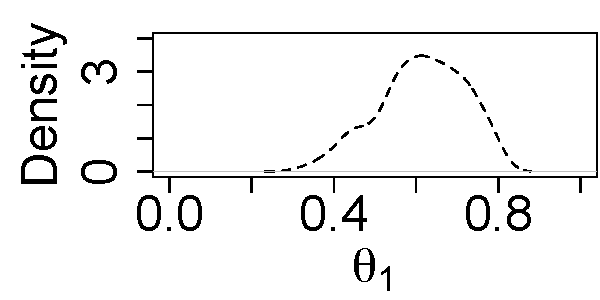
\includegraphics[scale=.3]{sims-10-1.pdf}}</span></td>
      </tr>
      <tr>
        <td id="L110" class="blob-num js-line-number" data-line-number="110"></td>
        <td id="LC110" class="blob-code blob-code-inner js-file-line">  &amp; <span class="pl-c1">\pbox</span>[c]{<span class="pl-c1">\textwidth</span>}{<span class="pl-c1">\includegraphics</span>[scale=.3]{sims-R-10-1.pdf}}</td>
      </tr>
      <tr>
        <td id="L111" class="blob-num js-line-number" data-line-number="111"></td>
        <td id="LC111" class="blob-code blob-code-inner js-file-line"><span class="pl-c1">\\</span></td>
      </tr>
      <tr>
        <td id="L112" class="blob-num js-line-number" data-line-number="112"></td>
        <td id="LC112" class="blob-code blob-code-inner js-file-line">  <span class="pl-s"><span class="pl-pds">$</span>N=<span class="pl-c1">100</span><span class="pl-pds">$</span></span> &amp; <span class="pl-c1">\pbox</span>[c]{<span class="pl-c1">\textwidth</span>}{<span class="pl-c1">\includegraphics</span>[scale=.3]{sims-R-1-2.pdf}}</td>
      </tr>
      <tr>
        <td id="L113" class="blob-num js-line-number" data-line-number="113"></td>
        <td id="LC113" class="blob-code blob-code-inner js-file-line"><span class="pl-c">%    &amp; \pbox[c]{\textwidth}{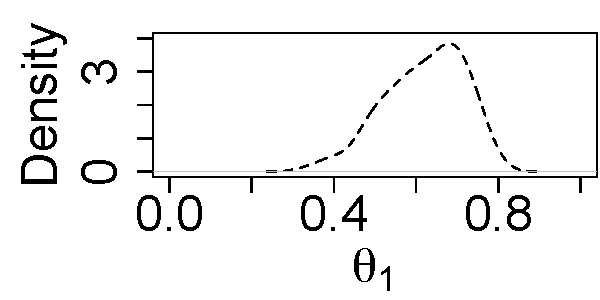
\includegraphics[scale=.3]{sims-10-2.pdf}}</span></td>
      </tr>
      <tr>
        <td id="L114" class="blob-num js-line-number" data-line-number="114"></td>
        <td id="LC114" class="blob-code blob-code-inner js-file-line">  &amp; <span class="pl-c1">\pbox</span>[c]{<span class="pl-c1">\textwidth</span>}{<span class="pl-c1">\includegraphics</span>[scale=.3]{sims-R-10-2.pdf}}</td>
      </tr>
      <tr>
        <td id="L115" class="blob-num js-line-number" data-line-number="115"></td>
        <td id="LC115" class="blob-code blob-code-inner js-file-line"><span class="pl-c1">\\</span></td>
      </tr>
      <tr>
        <td id="L116" class="blob-num js-line-number" data-line-number="116"></td>
        <td id="LC116" class="blob-code blob-code-inner js-file-line">  <span class="pl-s"><span class="pl-pds">$</span>N=<span class="pl-c1">200</span><span class="pl-pds">$</span></span> &amp; <span class="pl-c1">\pbox</span>[c]{<span class="pl-c1">\textwidth</span>}{<span class="pl-c1">\includegraphics</span>[scale=.3]{sims-R-1-3.pdf}}</td>
      </tr>
      <tr>
        <td id="L117" class="blob-num js-line-number" data-line-number="117"></td>
        <td id="LC117" class="blob-code blob-code-inner js-file-line"><span class="pl-c">%    &amp; \pbox[c]{\textwidth}{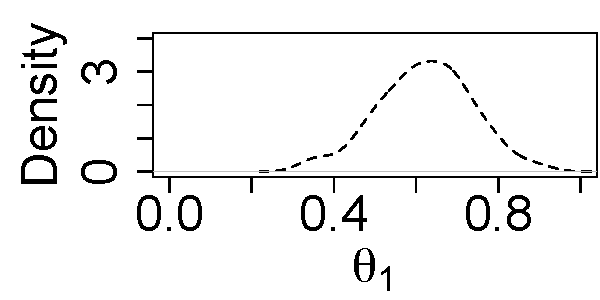
\includegraphics[scale=.3]{sims-10-3.pdf}}</span></td>
      </tr>
      <tr>
        <td id="L118" class="blob-num js-line-number" data-line-number="118"></td>
        <td id="LC118" class="blob-code blob-code-inner js-file-line">  &amp; <span class="pl-c1">\pbox</span>[c]{<span class="pl-c1">\textwidth</span>}{<span class="pl-c1">\includegraphics</span>[scale=.3]{sims-R-10-3.pdf}}</td>
      </tr>
      <tr>
        <td id="L119" class="blob-num js-line-number" data-line-number="119"></td>
        <td id="LC119" class="blob-code blob-code-inner js-file-line"><span class="pl-c1">\\</span></td>
      </tr>
      <tr>
        <td id="L120" class="blob-num js-line-number" data-line-number="120"></td>
        <td id="LC120" class="blob-code blob-code-inner js-file-line">  <span class="pl-s"><span class="pl-pds">$</span>N=<span class="pl-c1">500</span><span class="pl-pds">$</span></span> &amp; <span class="pl-c1">\pbox</span>[c]{<span class="pl-c1">\textwidth</span>}{<span class="pl-c1">\includegraphics</span>[scale=.3]{sims-R-1-4.pdf}}</td>
      </tr>
      <tr>
        <td id="L121" class="blob-num js-line-number" data-line-number="121"></td>
        <td id="LC121" class="blob-code blob-code-inner js-file-line"><span class="pl-c">%    &amp; \pbox[c]{\textwidth}{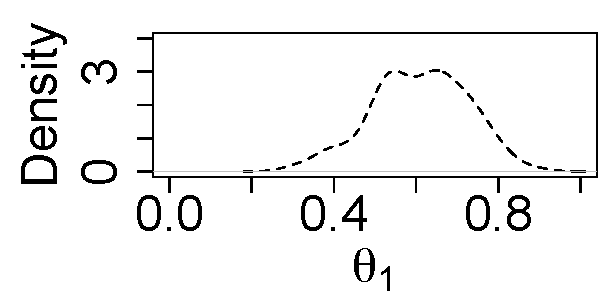
\includegraphics[scale=.3]{sims-10-4.pdf}}</span></td>
      </tr>
      <tr>
        <td id="L122" class="blob-num js-line-number" data-line-number="122"></td>
        <td id="LC122" class="blob-code blob-code-inner js-file-line">  &amp; <span class="pl-c1">\pbox</span>[c]{<span class="pl-c1">\textwidth</span>}{<span class="pl-c1">\includegraphics</span>[scale=.3]{sims-R-10-4.pdf}}</td>
      </tr>
      <tr>
        <td id="L123" class="blob-num js-line-number" data-line-number="123"></td>
        <td id="LC123" class="blob-code blob-code-inner js-file-line">
</td>
      </tr>
      <tr>
        <td id="L124" class="blob-num js-line-number" data-line-number="124"></td>
        <td id="LC124" class="blob-code blob-code-inner js-file-line">  </td>
      </tr>
      <tr>
        <td id="L125" class="blob-num js-line-number" data-line-number="125"></td>
        <td id="LC125" class="blob-code blob-code-inner js-file-line">  <span class="pl-c1">\end</span>{tabular}</td>
      </tr>
      <tr>
        <td id="L126" class="blob-num js-line-number" data-line-number="126"></td>
        <td id="LC126" class="blob-code blob-code-inner js-file-line"><span class="pl-c1">\end</span>{center}</td>
      </tr>
      <tr>
        <td id="L127" class="blob-num js-line-number" data-line-number="127"></td>
        <td id="LC127" class="blob-code blob-code-inner js-file-line"><span class="pl-c1">\caption</span>{{<span class="pl-c1">\footnotesize</span> Simulated distribution of binomial ordering preferences for a single expression type with <span class="pl-s"><span class="pl-pds">$</span><span class="pl-c1">\mu</span>=<span class="pl-c1">0.6</span><span class="pl-pds">$</span></span> in a standard 2-Alternative Iterated Learning Model (dotted lines) and one with an explicit regularization bias in data production of <span class="pl-s"><span class="pl-pds">$</span><span class="pl-c1">\alpha</span>=<span class="pl-c1">1.1</span><span class="pl-pds">$</span></span> (solid lines). Note that <span class="pl-s"><span class="pl-pds">$</span><span class="pl-c1">\theta</span>&#39;_<span class="pl-c1">1</span>=<span class="pl-c1">\theta</span>_<span class="pl-c1">1</span><span class="pl-pds">$</span></span> in the standard model. Regularization depends upon <span class="pl-s"><span class="pl-pds">$</span>N<span class="pl-pds">$</span></span> only in the model with an explicit regularization bias.}}</td>
      </tr>
      <tr>
        <td id="L128" class="blob-num js-line-number" data-line-number="128"></td>
        <td id="LC128" class="blob-code blob-code-inner js-file-line"><span class="pl-c1">\label</span>{fig:R11} </td>
      </tr>
      <tr>
        <td id="L129" class="blob-num js-line-number" data-line-number="129"></td>
        <td id="LC129" class="blob-code blob-code-inner js-file-line"><span class="pl-c1">\end</span>{figure}</td>
      </tr>
      <tr>
        <td id="L130" class="blob-num js-line-number" data-line-number="130"></td>
        <td id="LC130" class="blob-code blob-code-inner js-file-line">
</td>
      </tr>
      <tr>
        <td id="L131" class="blob-num js-line-number" data-line-number="131"></td>
        <td id="LC131" class="blob-code blob-code-inner js-file-line"><span class="pl-c">%\setlength\tabcolsep{1pt}</span></td>
      </tr>
      <tr>
        <td id="L132" class="blob-num js-line-number" data-line-number="132"></td>
        <td id="LC132" class="blob-code blob-code-inner js-file-line"><span class="pl-c">%\begin{figure}[ht]</span></td>
      </tr>
      <tr>
        <td id="L133" class="blob-num js-line-number" data-line-number="133"></td>
        <td id="LC133" class="blob-code blob-code-inner js-file-line"><span class="pl-c">%\begin{center}</span></td>
      </tr>
      <tr>
        <td id="L134" class="blob-num js-line-number" data-line-number="134"></td>
        <td id="LC134" class="blob-code blob-code-inner js-file-line"><span class="pl-c">%  \begin{tabular}{lcc}</span></td>
      </tr>
      <tr>
        <td id="L135" class="blob-num js-line-number" data-line-number="135"></td>
        <td id="LC135" class="blob-code blob-code-inner js-file-line"><span class="pl-c">% &amp; $\nu = 1$ &amp; $\nu = 10$</span></td>
      </tr>
      <tr>
        <td id="L136" class="blob-num js-line-number" data-line-number="136"></td>
        <td id="LC136" class="blob-code blob-code-inner js-file-line"><span class="pl-c">%  \\</span></td>
      </tr>
      <tr>
        <td id="L137" class="blob-num js-line-number" data-line-number="137"></td>
        <td id="LC137" class="blob-code blob-code-inner js-file-line"><span class="pl-c">%  $N=10$ &amp; \pbox[c]{\textwidth}{\includegraphics[scale=.3]{sims-1-1.pdf}}</span></td>
      </tr>
      <tr>
        <td id="L138" class="blob-num js-line-number" data-line-number="138"></td>
        <td id="LC138" class="blob-code blob-code-inner js-file-line"><span class="pl-c">%  &amp; \pbox[c]{\textwidth}{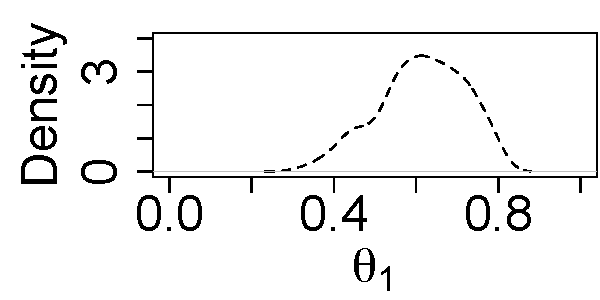
\includegraphics[scale=.3]{sims-10-1.pdf}}</span></td>
      </tr>
      <tr>
        <td id="L139" class="blob-num js-line-number" data-line-number="139"></td>
        <td id="LC139" class="blob-code blob-code-inner js-file-line"><span class="pl-c">%\\</span></td>
      </tr>
      <tr>
        <td id="L140" class="blob-num js-line-number" data-line-number="140"></td>
        <td id="LC140" class="blob-code blob-code-inner js-file-line"><span class="pl-c">%  $N=100$ &amp; \pbox[c]{\textwidth}{\includegraphics[scale=.3]{sims-1-2.pdf}}</span></td>
      </tr>
      <tr>
        <td id="L141" class="blob-num js-line-number" data-line-number="141"></td>
        <td id="LC141" class="blob-code blob-code-inner js-file-line"><span class="pl-c">%  &amp; \pbox[c]{\textwidth}{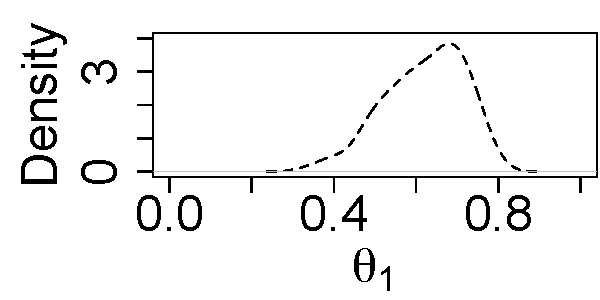
\includegraphics[scale=.3]{sims-10-2.pdf}}</span></td>
      </tr>
      <tr>
        <td id="L142" class="blob-num js-line-number" data-line-number="142"></td>
        <td id="LC142" class="blob-code blob-code-inner js-file-line"><span class="pl-c">%\\</span></td>
      </tr>
      <tr>
        <td id="L143" class="blob-num js-line-number" data-line-number="143"></td>
        <td id="LC143" class="blob-code blob-code-inner js-file-line"><span class="pl-c">%  $N=200$ &amp; \pbox[c]{\textwidth}{\includegraphics[scale=.3]{sims-1-3.pdf}}</span></td>
      </tr>
      <tr>
        <td id="L144" class="blob-num js-line-number" data-line-number="144"></td>
        <td id="LC144" class="blob-code blob-code-inner js-file-line"><span class="pl-c">%  &amp; \pbox[c]{\textwidth}{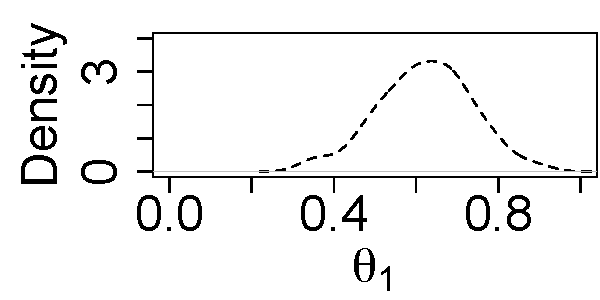
\includegraphics[scale=.3]{sims-10-3.pdf}}</span></td>
      </tr>
      <tr>
        <td id="L145" class="blob-num js-line-number" data-line-number="145"></td>
        <td id="LC145" class="blob-code blob-code-inner js-file-line"><span class="pl-c">%\\</span></td>
      </tr>
      <tr>
        <td id="L146" class="blob-num js-line-number" data-line-number="146"></td>
        <td id="LC146" class="blob-code blob-code-inner js-file-line"><span class="pl-c">%  $N=500$ &amp; \pbox[c]{\textwidth}{\includegraphics[scale=.3]{sims-1-4.pdf}}</span></td>
      </tr>
      <tr>
        <td id="L147" class="blob-num js-line-number" data-line-number="147"></td>
        <td id="LC147" class="blob-code blob-code-inner js-file-line"><span class="pl-c">%  &amp; \pbox[c]{\textwidth}{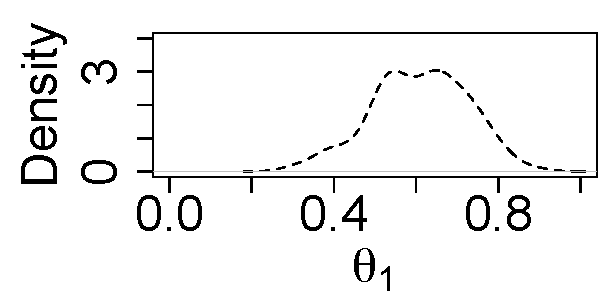
\includegraphics[scale=.3]{sims-10-4.pdf}}</span></td>
      </tr>
      <tr>
        <td id="L148" class="blob-num js-line-number" data-line-number="148"></td>
        <td id="LC148" class="blob-code blob-code-inner js-file-line"><span class="pl-c">%\\</span></td>
      </tr>
      <tr>
        <td id="L149" class="blob-num js-line-number" data-line-number="149"></td>
        <td id="LC149" class="blob-code blob-code-inner js-file-line"><span class="pl-c">%</span></td>
      </tr>
      <tr>
        <td id="L150" class="blob-num js-line-number" data-line-number="150"></td>
        <td id="LC150" class="blob-code blob-code-inner js-file-line"><span class="pl-c">%  </span></td>
      </tr>
      <tr>
        <td id="L151" class="blob-num js-line-number" data-line-number="151"></td>
        <td id="LC151" class="blob-code blob-code-inner js-file-line"><span class="pl-c">%  \end{tabular}</span></td>
      </tr>
      <tr>
        <td id="L152" class="blob-num js-line-number" data-line-number="152"></td>
        <td id="LC152" class="blob-code blob-code-inner js-file-line"><span class="pl-c">%\end{center}</span></td>
      </tr>
      <tr>
        <td id="L153" class="blob-num js-line-number" data-line-number="153"></td>
        <td id="LC153" class="blob-code blob-code-inner js-file-line"><span class="pl-c">%\caption{{\footnotesize Distribution of binomial ordering preferences in a standard 2-Alternative Iterated Learning Model \label{fig:R1}}}</span></td>
      </tr>
      <tr>
        <td id="L154" class="blob-num js-line-number" data-line-number="154"></td>
        <td id="LC154" class="blob-code blob-code-inner js-file-line"><span class="pl-c">%\end{figure}</span></td>
      </tr>
      <tr>
        <td id="L155" class="blob-num js-line-number" data-line-number="155"></td>
        <td id="LC155" class="blob-code blob-code-inner js-file-line">
</td>
      </tr>
      <tr>
        <td id="L156" class="blob-num js-line-number" data-line-number="156"></td>
        <td id="LC156" class="blob-code blob-code-inner js-file-line"><span class="pl-c1">\section</span>{Emergence of Frequency-Dependent Regularization in Iterated Learning}</td>
      </tr>
      <tr>
        <td id="L157" class="blob-num js-line-number" data-line-number="157"></td>
        <td id="LC157" class="blob-code blob-code-inner js-file-line"><span class="pl-c1">\label</span>{sec:emerg-freq-depend}</td>
      </tr>
      <tr>
        <td id="L158" class="blob-num js-line-number" data-line-number="158"></td>
        <td id="LC158" class="blob-code blob-code-inner js-file-line"><span class="pl-c">%</span></td>
      </tr>
      <tr>
        <td id="L159" class="blob-num js-line-number" data-line-number="159"></td>
        <td id="LC159" class="blob-code blob-code-inner js-file-line">The standard 2-Alternative Iterated Learning Model does not predict frequency-dependent regularization. We now demonstrate that we can predict frequency-dependent regularization by introducing a frequency-<span class="pl-c1">\emph</span>{independent} regularization bias into our model. Under this model, frequency-dependent regularization is an emergent property of the interaction of the frequency-independent regularization bias with the bottleneck effect of cultural transmission.</td>
      </tr>
      <tr>
        <td id="L160" class="blob-num js-line-number" data-line-number="160"></td>
        <td id="LC160" class="blob-code blob-code-inner js-file-line">
</td>
      </tr>
      <tr>
        <td id="L161" class="blob-num js-line-number" data-line-number="161"></td>
        <td id="LC161" class="blob-code blob-code-inner js-file-line">
</td>
      </tr>
      <tr>
        <td id="L162" class="blob-num js-line-number" data-line-number="162"></td>
        <td id="LC162" class="blob-code blob-code-inner js-file-line">We augment the learning and transmission process as follows. After hearing data, the learner chooses a hypothesis <span class="pl-s"><span class="pl-pds">$</span><span class="pl-c1">\theta</span>_<span class="pl-c1">1</span><span class="pl-pds">$</span></span> as before, then applies a regularization function to produce a new hypothesis <span class="pl-s"><span class="pl-pds">$</span><span class="pl-c1">\theta</span>_<span class="pl-c1">1</span>&#39;<span class="pl-pds">$</span></span>, then generates data from <span class="pl-s"><span class="pl-pds">$</span><span class="pl-c1">\theta</span>_<span class="pl-c1">1</span>&#39;<span class="pl-pds">$</span></span>.</td>
      </tr>
      <tr>
        <td id="L163" class="blob-num js-line-number" data-line-number="163"></td>
        <td id="LC163" class="blob-code blob-code-inner js-file-line">
</td>
      </tr>
      <tr>
        <td id="L164" class="blob-num js-line-number" data-line-number="164"></td>
        <td id="LC164" class="blob-code blob-code-inner js-file-line">The regularization function is the regularized incomplete beta function (equivalently, the cumulative distribution function of the beta distribution), restricted to be symmetric such that it has a single free parameter <span class="pl-s"><span class="pl-pds">$</span><span class="pl-c1">\alpha</span><span class="pl-pds">$</span></span>:</td>
      </tr>
      <tr>
        <td id="L165" class="blob-num js-line-number" data-line-number="165"></td>
        <td id="LC165" class="blob-code blob-code-inner js-file-line"><span class="pl-c1">\begin</span>{equation}</td>
      </tr>
      <tr>
        <td id="L166" class="blob-num js-line-number" data-line-number="166"></td>
        <td id="LC166" class="blob-code blob-code-inner js-file-line">f(x;<span class="pl-c1">\alpha</span>) = <span class="pl-c1">\frac</span>{<span class="pl-c1">\int</span>_0^{x}t^{<span class="pl-c1">\alpha</span>-1}(1-t)^{<span class="pl-c1">\alpha</span>-1}<span class="pl-cce">\,</span><span class="pl-c1">\mathrm</span>{d}t}{<span class="pl-c1">\mathrm</span>{B}(<span class="pl-c1">\alpha</span>,<span class="pl-c1">\alpha</span>)}</td>
      </tr>
      <tr>
        <td id="L167" class="blob-num js-line-number" data-line-number="167"></td>
        <td id="LC167" class="blob-code blob-code-inner js-file-line"><span class="pl-c1">\end</span>{equation}</td>
      </tr>
      <tr>
        <td id="L168" class="blob-num js-line-number" data-line-number="168"></td>
        <td id="LC168" class="blob-code blob-code-inner js-file-line">As shown in Fig.<span class="pl-cce">\ </span><span class="pl-c1">\ref</span>{fig:R}, the bias parameter <span class="pl-s"><span class="pl-pds">$</span><span class="pl-c1">\alpha</span><span class="pl-pds">$</span></span> controls strength of regularization. When <span class="pl-s"><span class="pl-pds">$</span><span class="pl-c1">\alpha</span>=<span class="pl-c1">1</span><span class="pl-pds">$</span></span>, this is the identity function, i.e.<span class="pl-cce">\ </span>no explicit regularization is added. As <span class="pl-s"><span class="pl-pds">$</span><span class="pl-c1">\alpha</span><span class="pl-pds">$</span></span> increases, the regularization bias grows stronger. </td>
      </tr>
      <tr>
        <td id="L169" class="blob-num js-line-number" data-line-number="169"></td>
        <td id="LC169" class="blob-code blob-code-inner js-file-line">
</td>
      </tr>
      <tr>
        <td id="L170" class="blob-num js-line-number" data-line-number="170"></td>
        <td id="LC170" class="blob-code blob-code-inner js-file-line"> <span class="pl-c1">\begin</span>{wrapfigure}{L}{0.35<span class="pl-c1">\textwidth</span>}</td>
      </tr>
      <tr>
        <td id="L171" class="blob-num js-line-number" data-line-number="171"></td>
        <td id="LC171" class="blob-code blob-code-inner js-file-line"><span class="pl-c">% \begin{figure}[ht]</span></td>
      </tr>
      <tr>
        <td id="L172" class="blob-num js-line-number" data-line-number="172"></td>
        <td id="LC172" class="blob-code blob-code-inner js-file-line"><span class="pl-c1">\begin</span>{center}</td>
      </tr>
      <tr>
        <td id="L173" class="blob-num js-line-number" data-line-number="173"></td>
        <td id="LC173" class="blob-code blob-code-inner js-file-line"><span class="pl-c1">\includegraphics</span>[scale=.2]{R.pdf}</td>
      </tr>
      <tr>
        <td id="L174" class="blob-num js-line-number" data-line-number="174"></td>
        <td id="LC174" class="blob-code blob-code-inner js-file-line"><span class="pl-c1">\end</span>{center}</td>
      </tr>
      <tr>
        <td id="L175" class="blob-num js-line-number" data-line-number="175"></td>
        <td id="LC175" class="blob-code blob-code-inner js-file-line"><span class="pl-c1">\caption</span>{{<span class="pl-c1">\footnotesize</span> Regularization function with different values of <span class="pl-s"><span class="pl-pds">$</span><span class="pl-c1">\alpha</span><span class="pl-pds">$</span></span> <span class="pl-c1">\label</span>{fig:R}}}</td>
      </tr>
      <tr>
        <td id="L176" class="blob-num js-line-number" data-line-number="176"></td>
        <td id="LC176" class="blob-code blob-code-inner js-file-line"><span class="pl-c1">\end</span>{wrapfigure}</td>
      </tr>
      <tr>
        <td id="L177" class="blob-num js-line-number" data-line-number="177"></td>
        <td id="LC177" class="blob-code blob-code-inner js-file-line">
</td>
      </tr>
      <tr>
        <td id="L178" class="blob-num js-line-number" data-line-number="178"></td>
        <td id="LC178" class="blob-code blob-code-inner js-file-line"> <span class="pl-c1">\subsection</span>{Results: Frequency-dependent regularization}</td>
      </tr>
      <tr>
        <td id="L179" class="blob-num js-line-number" data-line-number="179"></td>
        <td id="LC179" class="blob-code blob-code-inner js-file-line"> When we repeat the simulations from above using  a non-trivial regularization bias <span class="pl-s"><span class="pl-pds">$</span><span class="pl-c1">\alpha</span>=<span class="pl-c1">1.1</span><span class="pl-pds">$</span></span>, we see frequency-dependent regularization in the case with a dense prior (Fig.<span class="pl-cce">\ </span><span class="pl-c1">\ref</span>{fig:R11}). Although the regularization bias itself is frequency-independent, frequency-dependence emerges from the interaction of the regularization bias with the process of cultural transmission: At lower frequencies, there is not sufficient data for the regularization bias to overcome the prior. At higher frequencies, the regularization bias becomes increasingly dominant as there is increasingly enough data for the effects of this bias to be carried across generations. Even a relatively weak bias (<span class="pl-s"><span class="pl-pds">$</span><span class="pl-c1">\alpha</span>=<span class="pl-c1">1.1</span><span class="pl-pds">$</span></span>) can produce noticeable regularization when compounded across generations. However, the prior always continues to exert some influence; thus, even the highest frequency expressions do not become completely regularized.</td>
      </tr>
      <tr>
        <td id="L180" class="blob-num js-line-number" data-line-number="180"></td>
        <td id="LC180" class="blob-code blob-code-inner js-file-line"> </td>
      </tr>
      <tr>
        <td id="L181" class="blob-num js-line-number" data-line-number="181"></td>
        <td id="LC181" class="blob-code blob-code-inner js-file-line"> Another linguistically accurate property of this model is that for sufficiently high values of <span class="pl-s"><span class="pl-pds">$</span>N<span class="pl-pds">$</span></span>, the distribution over hypotheses includes a mode on the opposite side of 0.5 from the prior. Thus the model correctly predicts that at high enough frequencies, an expression can become idiosyncratically preferred in the opposite of its compositionally predicted direction (as in ``ladies and gentlemen&#39;&#39;).</td>
      </tr>
      <tr>
        <td id="L182" class="blob-num js-line-number" data-line-number="182"></td>
        <td id="LC182" class="blob-code blob-code-inner js-file-line"> </td>
      </tr>
      <tr>
        <td id="L183" class="blob-num js-line-number" data-line-number="183"></td>
        <td id="LC183" class="blob-code blob-code-inner js-file-line">
</td>
      </tr>
      <tr>
        <td id="L184" class="blob-num js-line-number" data-line-number="184"></td>
        <td id="LC184" class="blob-code blob-code-inner js-file-line"><span class="pl-c1">\subsection</span>{Results: Simulating corpus data}<span class="pl-c1">\label</span>{corpus}</td>
      </tr>
      <tr>
        <td id="L185" class="blob-num js-line-number" data-line-number="185"></td>
        <td id="LC185" class="blob-code blob-code-inner js-file-line">Having demonstrated that our augmented model produces frequency-dependent regularization, we now show that it additionally predicts the true language-wide distribution of binomial preference strengths seen in corpus data. The target distribution to be accounted for is shown in Fig.<span class="pl-cce">\ </span><span class="pl-c1">\ref</span>{fig:corpus}.</td>
      </tr>
      <tr>
        <td id="L186" class="blob-num js-line-number" data-line-number="186"></td>
        <td id="LC186" class="blob-code blob-code-inner js-file-line">
</td>
      </tr>
      <tr>
        <td id="L187" class="blob-num js-line-number" data-line-number="187"></td>
        <td id="LC187" class="blob-code blob-code-inner js-file-line">
</td>
      </tr>
      <tr>
        <td id="L188" class="blob-num js-line-number" data-line-number="188"></td>
        <td id="LC188" class="blob-code blob-code-inner js-file-line">We take the true properties of each binomial expression in the corpus: its compositional preference determines <span class="pl-s"><span class="pl-pds">$</span><span class="pl-c1">\mu</span><span class="pl-pds">$</span></span> and its overall frequency determines <span class="pl-s"><span class="pl-pds">$</span>N<span class="pl-pds">$</span></span>. We scale overall frequency counts based on estimated lifetime exposure to 300 million total words (<span class="pl-c1">\citeNP</span>[footnote 10]{Levy:2012bj}). The resulting distribution of values <span class="pl-s"><span class="pl-pds">$</span>N<span class="pl-pds">$</span></span> is shown in Fig.<span class="pl-cce">\ </span><span class="pl-c1">\ref</span>{fig:extremity}. For each binomial in the corpus, we approximate the stationary distribution by modeling 10 chains of learners for 200 generations each and take the hypothesis <span class="pl-s"><span class="pl-pds">$</span><span class="pl-c1">\theta</span>&#39;_<span class="pl-c1">1</span><span class="pl-pds">$</span></span> of the final generation of each chain.</td>
      </tr>
      <tr>
        <td id="L189" class="blob-num js-line-number" data-line-number="189"></td>
        <td id="LC189" class="blob-code blob-code-inner js-file-line">
</td>
      </tr>
      <tr>
        <td id="L190" class="blob-num js-line-number" data-line-number="190"></td>
        <td id="LC190" class="blob-code blob-code-inner js-file-line"><span class="pl-c">% \begin{figure}[ht]</span></td>
      </tr>
      <tr>
        <td id="L191" class="blob-num js-line-number" data-line-number="191"></td>
        <td id="LC191" class="blob-code blob-code-inner js-file-line"><span class="pl-c">%%\begin{wrapfigure}[14]{L}{0.5\textwidth}</span></td>
      </tr>
      <tr>
        <td id="L192" class="blob-num js-line-number" data-line-number="192"></td>
        <td id="LC192" class="blob-code blob-code-inner js-file-line"><span class="pl-c">%\begin{center}</span></td>
      </tr>
      <tr>
        <td id="L193" class="blob-num js-line-number" data-line-number="193"></td>
        <td id="LC193" class="blob-code blob-code-inner js-file-line"><span class="pl-c">%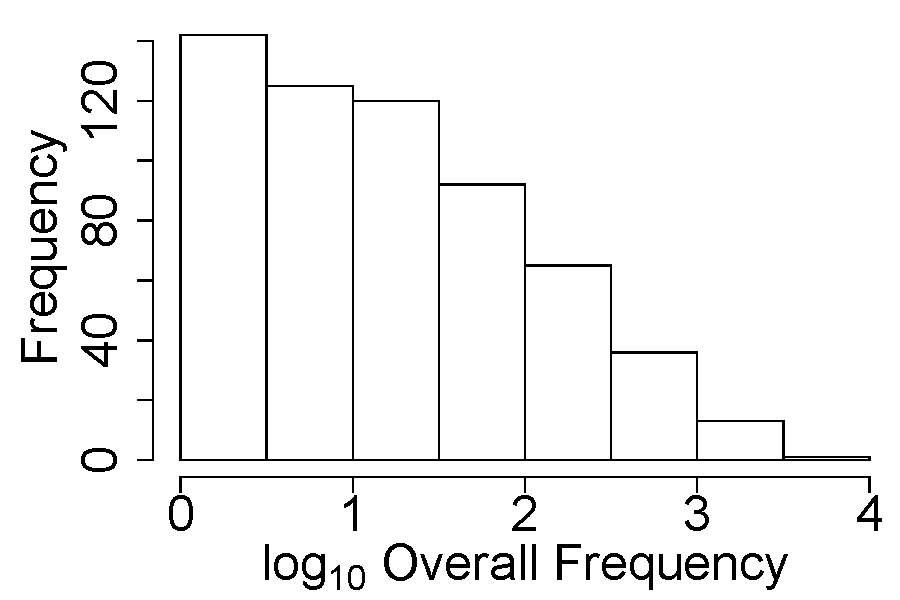
\includegraphics[scale=.25]{N-hist.pdf}</span></td>
      </tr>
      <tr>
        <td id="L194" class="blob-num js-line-number" data-line-number="194"></td>
        <td id="LC194" class="blob-code blob-code-inner js-file-line"><span class="pl-c">%\end{center}</span></td>
      </tr>
      <tr>
        <td id="L195" class="blob-num js-line-number" data-line-number="195"></td>
        <td id="LC195" class="blob-code blob-code-inner js-file-line"><span class="pl-c">%\caption{{\footnotesize The distribution over overall frequencies $N$ is non-Zipfian because Morgan and Levy&#39;s corpus is restricted to binomial types with at least 1000 occurrences in the Google Books corpus in order to ensure that they have reliable relative frequency estimates. \label{fig:N}}}</span></td>
      </tr>
      <tr>
        <td id="L196" class="blob-num js-line-number" data-line-number="196"></td>
        <td id="LC196" class="blob-code blob-code-inner js-file-line"><span class="pl-c">%\end{figure}</span></td>
      </tr>
      <tr>
        <td id="L197" class="blob-num js-line-number" data-line-number="197"></td>
        <td id="LC197" class="blob-code blob-code-inner js-file-line">
</td>
      </tr>
      <tr>
        <td id="L198" class="blob-num js-line-number" data-line-number="198"></td>
        <td id="LC198" class="blob-code blob-code-inner js-file-line"><span class="pl-c">% \begin{SCfigure}</span></td>
      </tr>
      <tr>
        <td id="L199" class="blob-num js-line-number" data-line-number="199"></td>
        <td id="LC199" class="blob-code blob-code-inner js-file-line"><span class="pl-c">%\centering</span></td>
      </tr>
      <tr>
        <td id="L200" class="blob-num js-line-number" data-line-number="200"></td>
        <td id="LC200" class="blob-code blob-code-inner js-file-line"><span class="pl-c">%\caption{{\footnotesize The distribution over overall frequencies $N$ is non-Zipfian because the corpus is restricted to binomial types with at least 1000 occurrences in the Google Books corpus. \label{fig:N}}}</span></td>
      </tr>
      <tr>
        <td id="L201" class="blob-num js-line-number" data-line-number="201"></td>
        <td id="LC201" class="blob-code blob-code-inner js-file-line"><span class="pl-c">%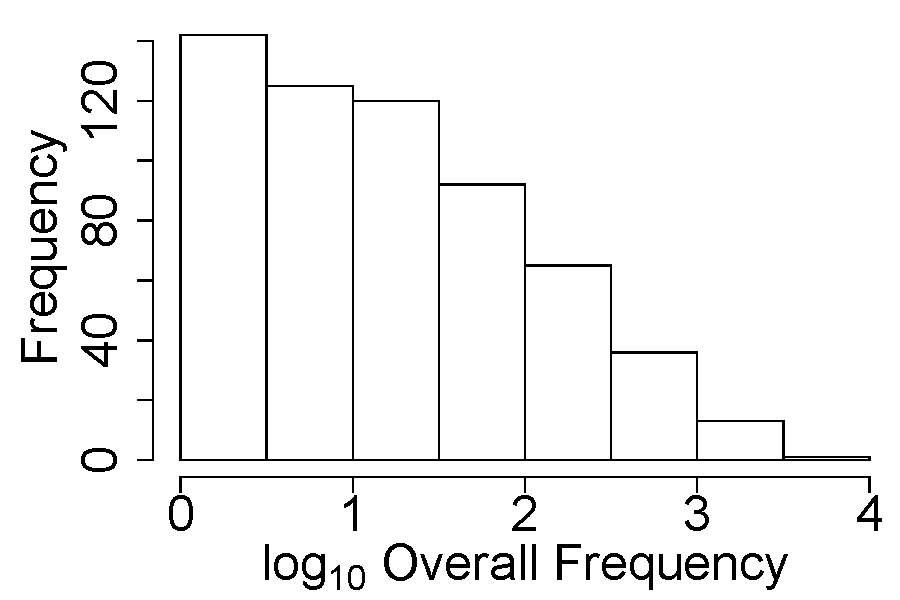
\includegraphics[scale=.25]{N-hist.pdf}</span></td>
      </tr>
      <tr>
        <td id="L202" class="blob-num js-line-number" data-line-number="202"></td>
        <td id="LC202" class="blob-code blob-code-inner js-file-line"><span class="pl-c">%\end{SCfigure}</span></td>
      </tr>
      <tr>
        <td id="L203" class="blob-num js-line-number" data-line-number="203"></td>
        <td id="LC203" class="blob-code blob-code-inner js-file-line">
</td>
      </tr>
      <tr>
        <td id="L204" class="blob-num js-line-number" data-line-number="204"></td>
        <td id="LC204" class="blob-code blob-code-inner js-file-line">Our model has two free parameters, $\nu$ and $\alpha$. We model the corpus data as described above for a range of values of both of these parameters. As shown in Fig.\ \ref{fig:nuxR}, our model displays a trade-off between the prior and the regularization bias as a function of these parameters. At appropriate values, our model correctly predicts the multimodal distribution of corpus data as seen in Fig.\ \ref{fig:corpus}.%\footnote{Why do we predict the \emph{distribution} of binomial expression preferences rather than the preferences for individual binomials? There is stochasticity in how any individual binomial will evolve over time: particularly for high frequency binomials, they can become polarized either in their compositionally preferred direction or non-preferred direction, as shown in Fig ?. We don&#39;t expect to be able to predict the individual historical quirks that lead individual items to freeze in one order or another, but we \emph{can} predict the distribution over preferences for items of a given prior $\mu$ with a given frequency $N$. It therefore makes sense for us to test our language-wide predictions against the language-wide distribution rather than testing predictions for any individual item.}</td>
      </tr>
      <tr>
        <td id="L205" class="blob-num js-line-number" data-line-number="205"></td>
        <td id="LC205" class="blob-code blob-code-inner js-file-line">
</td>
      </tr>
      <tr>
        <td id="L206" class="blob-num js-line-number" data-line-number="206"></td>
        <td id="LC206" class="blob-code blob-code-inner js-file-line">
</td>
      </tr>
      <tr>
        <td id="L207" class="blob-num js-line-number" data-line-number="207"></td>
        <td id="LC207" class="blob-code blob-code-inner js-file-line"><span class="pl-c1">\begin</span>{figure}[t]</td>
      </tr>
      <tr>
        <td id="L208" class="blob-num js-line-number" data-line-number="208"></td>
        <td id="LC208" class="blob-code blob-code-inner js-file-line"><span class="pl-c1">\setlength\tabcolsep</span>{1pt}</td>
      </tr>
      <tr>
        <td id="L209" class="blob-num js-line-number" data-line-number="209"></td>
        <td id="LC209" class="blob-code blob-code-inner js-file-line"><span class="pl-c1">\begin</span>{center}</td>
      </tr>
      <tr>
        <td id="L210" class="blob-num js-line-number" data-line-number="210"></td>
        <td id="LC210" class="blob-code blob-code-inner js-file-line"><span class="pl-c">%  \begin{tabular}{lccc}</span></td>
      </tr>
      <tr>
        <td id="L211" class="blob-num js-line-number" data-line-number="211"></td>
        <td id="LC211" class="blob-code blob-code-inner js-file-line"><span class="pl-c">% &amp; $\nu = 10$ &amp; $\nu = 15$ &amp; $\nu = 20$</span></td>
      </tr>
      <tr>
        <td id="L212" class="blob-num js-line-number" data-line-number="212"></td>
        <td id="LC212" class="blob-code blob-code-inner js-file-line"><span class="pl-c">%  \\</span></td>
      </tr>
      <tr>
        <td id="L213" class="blob-num js-line-number" data-line-number="213"></td>
        <td id="LC213" class="blob-code blob-code-inner js-file-line"><span class="pl-c">%  $\alpha=1$ &amp; \pbox[c]{\textwidth}{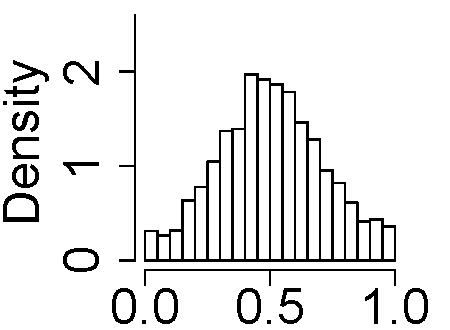
\includegraphics[scale=.3]{nu1R0.pdf}}</span></td>
      </tr>
      <tr>
        <td id="L214" class="blob-num js-line-number" data-line-number="214"></td>
        <td id="LC214" class="blob-code blob-code-inner js-file-line"><span class="pl-c">%  &amp; \pbox[c]{\textwidth}{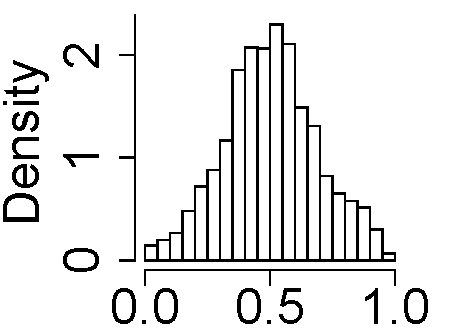
\includegraphics[scale=.3]{nu2R0.pdf}}</span></td>
      </tr>
      <tr>
        <td id="L215" class="blob-num js-line-number" data-line-number="215"></td>
        <td id="LC215" class="blob-code blob-code-inner js-file-line"><span class="pl-c">%  &amp; \pbox[c]{\textwidth}{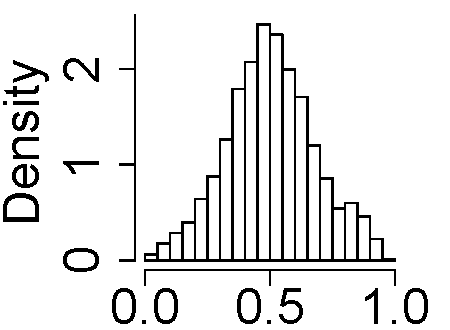
\includegraphics[scale=.3]{nu3R0.pdf}}</span></td>
      </tr>
      <tr>
        <td id="L216" class="blob-num js-line-number" data-line-number="216"></td>
        <td id="LC216" class="blob-code blob-code-inner js-file-line"><span class="pl-c">%</span></td>
      </tr>
      <tr>
        <td id="L217" class="blob-num js-line-number" data-line-number="217"></td>
        <td id="LC217" class="blob-code blob-code-inner js-file-line"><span class="pl-c">%  \\</span></td>
      </tr>
      <tr>
        <td id="L218" class="blob-num js-line-number" data-line-number="218"></td>
        <td id="LC218" class="blob-code blob-code-inner js-file-line"><span class="pl-c">%  $\alpha=1.1$ &amp; \pbox[c]{\textwidth}{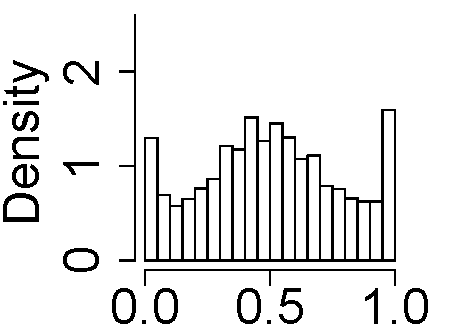
\includegraphics[scale=.3]{nu1R1.pdf}}</span></td>
      </tr>
      <tr>
        <td id="L219" class="blob-num js-line-number" data-line-number="219"></td>
        <td id="LC219" class="blob-code blob-code-inner js-file-line"><span class="pl-c">%  &amp; \pbox[c]{\textwidth}{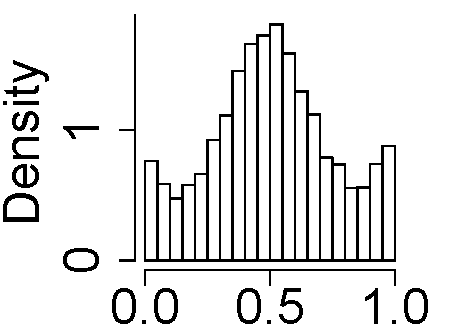
\includegraphics[scale=.3]{nu2R1.pdf}}</span></td>
      </tr>
      <tr>
        <td id="L220" class="blob-num js-line-number" data-line-number="220"></td>
        <td id="LC220" class="blob-code blob-code-inner js-file-line"><span class="pl-c">%  &amp; \pbox[c]{\textwidth}{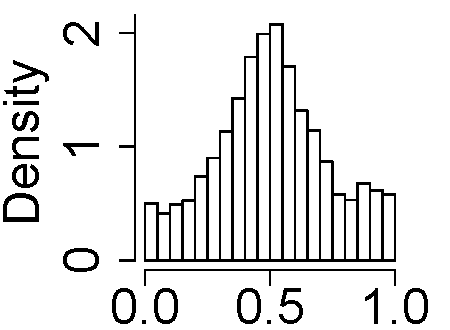
\includegraphics[scale=.3]{nu3R1.pdf}}</span></td>
      </tr>
      <tr>
        <td id="L221" class="blob-num js-line-number" data-line-number="221"></td>
        <td id="LC221" class="blob-code blob-code-inner js-file-line"><span class="pl-c">%%  &amp; \pbox[c]{\textwidth}{\includegraphics[scale=.3]{nu4R1.pdf}}</span></td>
      </tr>
      <tr>
        <td id="L222" class="blob-num js-line-number" data-line-number="222"></td>
        <td id="LC222" class="blob-code blob-code-inner js-file-line"><span class="pl-c">%</span></td>
      </tr>
      <tr>
        <td id="L223" class="blob-num js-line-number" data-line-number="223"></td>
        <td id="LC223" class="blob-code blob-code-inner js-file-line"><span class="pl-c">%  </span></td>
      </tr>
      <tr>
        <td id="L224" class="blob-num js-line-number" data-line-number="224"></td>
        <td id="LC224" class="blob-code blob-code-inner js-file-line"><span class="pl-c">%  \\</span></td>
      </tr>
      <tr>
        <td id="L225" class="blob-num js-line-number" data-line-number="225"></td>
        <td id="LC225" class="blob-code blob-code-inner js-file-line"><span class="pl-c">%  $\alpha=1.3$ &amp; \pbox[c]{\textwidth}{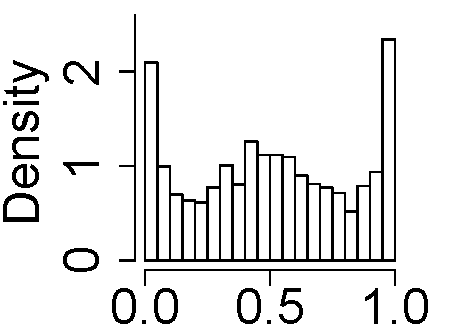
\includegraphics[scale=.3]{nu1R2.pdf}}</span></td>
      </tr>
      <tr>
        <td id="L226" class="blob-num js-line-number" data-line-number="226"></td>
        <td id="LC226" class="blob-code blob-code-inner js-file-line"><span class="pl-c">%  &amp; \pbox[c]{\textwidth}{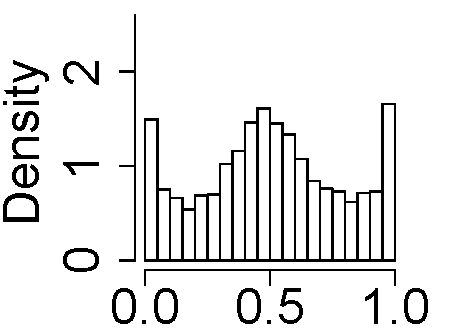
\includegraphics[scale=.3]{nu2R2.pdf}}</span></td>
      </tr>
      <tr>
        <td id="L227" class="blob-num js-line-number" data-line-number="227"></td>
        <td id="LC227" class="blob-code blob-code-inner js-file-line"><span class="pl-c">%  &amp; \pbox[c]{\textwidth}{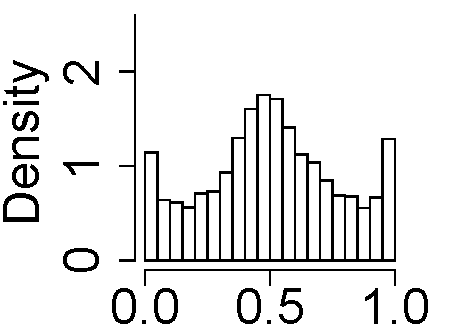
\includegraphics[scale=.3]{nu3R2.pdf}}</span></td>
      </tr>
      <tr>
        <td id="L228" class="blob-num js-line-number" data-line-number="228"></td>
        <td id="LC228" class="blob-code blob-code-inner js-file-line"><span class="pl-c">%%  &amp; \pbox[c]{\textwidth}{\includegraphics[scale=.3]{nu4R2.pdf}}</span></td>
      </tr>
      <tr>
        <td id="L229" class="blob-num js-line-number" data-line-number="229"></td>
        <td id="LC229" class="blob-code blob-code-inner js-file-line"><span class="pl-c">%</span></td>
      </tr>
      <tr>
        <td id="L230" class="blob-num js-line-number" data-line-number="230"></td>
        <td id="LC230" class="blob-code blob-code-inner js-file-line"><span class="pl-c">%  \\</span></td>
      </tr>
      <tr>
        <td id="L231" class="blob-num js-line-number" data-line-number="231"></td>
        <td id="LC231" class="blob-code blob-code-inner js-file-line"><span class="pl-c">%  $\alpha=1.5$ &amp; \pbox[c]{\textwidth}{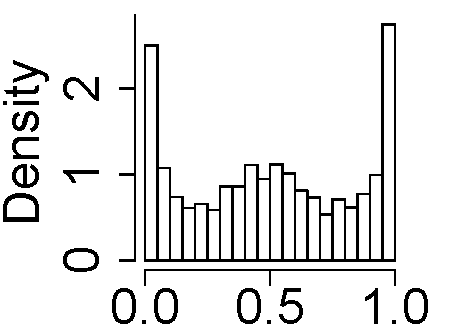
\includegraphics[scale=.3]{nu1R3.pdf}}</span></td>
      </tr>
      <tr>
        <td id="L232" class="blob-num js-line-number" data-line-number="232"></td>
        <td id="LC232" class="blob-code blob-code-inner js-file-line"><span class="pl-c">%  &amp; \pbox[c]{\textwidth}{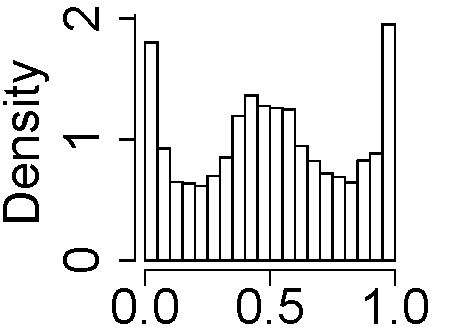
\includegraphics[scale=.3]{nu2R3.pdf}}</span></td>
      </tr>
      <tr>
        <td id="L233" class="blob-num js-line-number" data-line-number="233"></td>
        <td id="LC233" class="blob-code blob-code-inner js-file-line"><span class="pl-c">%  &amp; \pbox[c]{\textwidth}{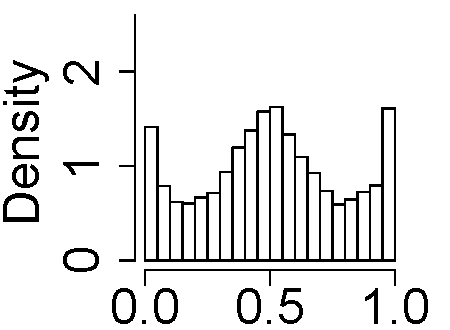
\includegraphics[scale=.3]{nu3R3.pdf}}</span></td>
      </tr>
      <tr>
        <td id="L234" class="blob-num js-line-number" data-line-number="234"></td>
        <td id="LC234" class="blob-code blob-code-inner js-file-line"><span class="pl-c">%%  &amp; \pbox[c]{\textwidth}{\includegraphics[scale=.3]{nu4R3.pdf}}</span></td>
      </tr>
      <tr>
        <td id="L235" class="blob-num js-line-number" data-line-number="235"></td>
        <td id="LC235" class="blob-code blob-code-inner js-file-line"><span class="pl-c">%</span></td>
      </tr>
      <tr>
        <td id="L236" class="blob-num js-line-number" data-line-number="236"></td>
        <td id="LC236" class="blob-code blob-code-inner js-file-line"><span class="pl-c">%</span></td>
      </tr>
      <tr>
        <td id="L237" class="blob-num js-line-number" data-line-number="237"></td>
        <td id="LC237" class="blob-code blob-code-inner js-file-line"><span class="pl-c">%  </span></td>
      </tr>
      <tr>
        <td id="L238" class="blob-num js-line-number" data-line-number="238"></td>
        <td id="LC238" class="blob-code blob-code-inner js-file-line"><span class="pl-c">%  \end{tabular}</span></td>
      </tr>
      <tr>
        <td id="L239" class="blob-num js-line-number" data-line-number="239"></td>
        <td id="LC239" class="blob-code blob-code-inner js-file-line">  </td>
      </tr>
      <tr>
        <td id="L240" class="blob-num js-line-number" data-line-number="240"></td>
        <td id="LC240" class="blob-code blob-code-inner js-file-line">    <span class="pl-c1">\begin</span>{tabular}{lcccc}</td>
      </tr>
      <tr>
        <td id="L241" class="blob-num js-line-number" data-line-number="241"></td>
        <td id="LC241" class="blob-code blob-code-inner js-file-line">    &amp; <span class="pl-s"><span class="pl-pds">$</span><span class="pl-c1">\alpha</span>=<span class="pl-c1">1</span><span class="pl-pds">$</span></span> &amp; <span class="pl-s"><span class="pl-pds">$</span><span class="pl-c1">\alpha</span>=<span class="pl-c1">1.1</span><span class="pl-pds">$</span></span> &amp; <span class="pl-s"><span class="pl-pds">$</span><span class="pl-c1">\alpha</span>=<span class="pl-c1">1.3</span><span class="pl-pds">$</span></span> &amp; <span class="pl-s"><span class="pl-pds">$</span><span class="pl-c1">\alpha</span>=<span class="pl-c1">1.5</span><span class="pl-pds">$</span></span></td>
      </tr>
      <tr>
        <td id="L242" class="blob-num js-line-number" data-line-number="242"></td>
        <td id="LC242" class="blob-code blob-code-inner js-file-line">  <span class="pl-c1">\\</span></td>
      </tr>
      <tr>
        <td id="L243" class="blob-num js-line-number" data-line-number="243"></td>
        <td id="LC243" class="blob-code blob-code-inner js-file-line">  <span class="pl-s"><span class="pl-pds">$</span><span class="pl-c1">\nu</span>=<span class="pl-c1">10</span><span class="pl-pds">$</span></span> &amp; <span class="pl-c1">\pbox</span>[c]{<span class="pl-c1">\textwidth</span>}{<span class="pl-c1">\includegraphics</span>[scale=.25]{nu1R0.pdf}} &amp;</td>
      </tr>
      <tr>
        <td id="L244" class="blob-num js-line-number" data-line-number="244"></td>
        <td id="LC244" class="blob-code blob-code-inner js-file-line"><span class="pl-c1">\pbox</span>[c]{<span class="pl-c1">\textwidth</span>}{<span class="pl-c1">\includegraphics</span>[scale=.25]{nu1R1.pdf}} &amp;</td>
      </tr>
      <tr>
        <td id="L245" class="blob-num js-line-number" data-line-number="245"></td>
        <td id="LC245" class="blob-code blob-code-inner js-file-line"><span class="pl-c1">\pbox</span>[c]{<span class="pl-c1">\textwidth</span>}{<span class="pl-c1">\includegraphics</span>[scale=.25]{nu1R2.pdf}} &amp;</td>
      </tr>
      <tr>
        <td id="L246" class="blob-num js-line-number" data-line-number="246"></td>
        <td id="LC246" class="blob-code blob-code-inner js-file-line"><span class="pl-c1">\pbox</span>[c]{<span class="pl-c1">\textwidth</span>}{<span class="pl-c1">\includegraphics</span>[scale=.25]{nu1R3.pdf}}</td>
      </tr>
      <tr>
        <td id="L247" class="blob-num js-line-number" data-line-number="247"></td>
        <td id="LC247" class="blob-code blob-code-inner js-file-line">
</td>
      </tr>
      <tr>
        <td id="L248" class="blob-num js-line-number" data-line-number="248"></td>
        <td id="LC248" class="blob-code blob-code-inner js-file-line">  <span class="pl-c1">\\</span></td>
      </tr>
      <tr>
        <td id="L249" class="blob-num js-line-number" data-line-number="249"></td>
        <td id="LC249" class="blob-code blob-code-inner js-file-line">  <span class="pl-s"><span class="pl-pds">$</span><span class="pl-c1">\nu</span>=<span class="pl-c1">15</span><span class="pl-pds">$</span></span> &amp; <span class="pl-c1">\pbox</span>[c]{<span class="pl-c1">\textwidth</span>}{<span class="pl-c1">\includegraphics</span>[scale=.25]{nu2R0.pdf}} &amp;</td>
      </tr>
      <tr>
        <td id="L250" class="blob-num js-line-number" data-line-number="250"></td>
        <td id="LC250" class="blob-code blob-code-inner js-file-line"><span class="pl-c1">\pbox</span>[c]{<span class="pl-c1">\textwidth</span>}{<span class="pl-c1">\includegraphics</span>[scale=.25]{nu2R1.pdf}} &amp;</td>
      </tr>
      <tr>
        <td id="L251" class="blob-num js-line-number" data-line-number="251"></td>
        <td id="LC251" class="blob-code blob-code-inner js-file-line"><span class="pl-c1">\pbox</span>[c]{<span class="pl-c1">\textwidth</span>}{<span class="pl-c1">\includegraphics</span>[scale=.25]{nu2R2.pdf}} &amp;</td>
      </tr>
      <tr>
        <td id="L252" class="blob-num js-line-number" data-line-number="252"></td>
        <td id="LC252" class="blob-code blob-code-inner js-file-line"><span class="pl-c1">\pbox</span>[c]{<span class="pl-c1">\textwidth</span>}{<span class="pl-c1">\includegraphics</span>[scale=.25]{nu2R3.pdf}}</td>
      </tr>
      <tr>
        <td id="L253" class="blob-num js-line-number" data-line-number="253"></td>
        <td id="LC253" class="blob-code blob-code-inner js-file-line">
</td>
      </tr>
      <tr>
        <td id="L254" class="blob-num js-line-number" data-line-number="254"></td>
        <td id="LC254" class="blob-code blob-code-inner js-file-line">  <span class="pl-c1">\\</span></td>
      </tr>
      <tr>
        <td id="L255" class="blob-num js-line-number" data-line-number="255"></td>
        <td id="LC255" class="blob-code blob-code-inner js-file-line">  <span class="pl-s"><span class="pl-pds">$</span><span class="pl-c1">\nu</span>=<span class="pl-c1">20</span><span class="pl-pds">$</span></span> &amp; <span class="pl-c1">\pbox</span>[c]{<span class="pl-c1">\textwidth</span>}{<span class="pl-c1">\includegraphics</span>[scale=.25]{nu3R0.pdf}} &amp;</td>
      </tr>
      <tr>
        <td id="L256" class="blob-num js-line-number" data-line-number="256"></td>
        <td id="LC256" class="blob-code blob-code-inner js-file-line"><span class="pl-c1">\pbox</span>[c]{<span class="pl-c1">\textwidth</span>}{<span class="pl-c1">\includegraphics</span>[scale=.25]{nu3R1.pdf}} &amp;</td>
      </tr>
      <tr>
        <td id="L257" class="blob-num js-line-number" data-line-number="257"></td>
        <td id="LC257" class="blob-code blob-code-inner js-file-line"><span class="pl-c1">\pbox</span>[c]{<span class="pl-c1">\textwidth</span>}{<span class="pl-c1">\includegraphics</span>[scale=.25]{nu3R2.pdf}} &amp;</td>
      </tr>
      <tr>
        <td id="L258" class="blob-num js-line-number" data-line-number="258"></td>
        <td id="LC258" class="blob-code blob-code-inner js-file-line"><span class="pl-c1">\pbox</span>[c]{<span class="pl-c1">\textwidth</span>}{<span class="pl-c1">\includegraphics</span>[scale=.25]{nu3R3.pdf}}</td>
      </tr>
      <tr>
        <td id="L259" class="blob-num js-line-number" data-line-number="259"></td>
        <td id="LC259" class="blob-code blob-code-inner js-file-line">
</td>
      </tr>
      <tr>
        <td id="L260" class="blob-num js-line-number" data-line-number="260"></td>
        <td id="LC260" class="blob-code blob-code-inner js-file-line">
</td>
      </tr>
      <tr>
        <td id="L261" class="blob-num js-line-number" data-line-number="261"></td>
        <td id="LC261" class="blob-code blob-code-inner js-file-line">  </td>
      </tr>
      <tr>
        <td id="L262" class="blob-num js-line-number" data-line-number="262"></td>
        <td id="LC262" class="blob-code blob-code-inner js-file-line">  <span class="pl-c1">\end</span>{tabular}</td>
      </tr>
      <tr>
        <td id="L263" class="blob-num js-line-number" data-line-number="263"></td>
        <td id="LC263" class="blob-code blob-code-inner js-file-line">  </td>
      </tr>
      <tr>
        <td id="L264" class="blob-num js-line-number" data-line-number="264"></td>
        <td id="LC264" class="blob-code blob-code-inner js-file-line"><span class="pl-c1">\end</span>{center}</td>
      </tr>
      <tr>
        <td id="L265" class="blob-num js-line-number" data-line-number="265"></td>
        <td id="LC265" class="blob-code blob-code-inner js-file-line"><span class="pl-c1">\caption</span>{{<span class="pl-c1">\footnotesize</span> Predicted distribution of <span class="pl-s"><span class="pl-pds">$</span><span class="pl-c1">\theta</span>&#39;_<span class="pl-c1">1</span><span class="pl-pds">$</span></span>. We see a trade-off between effects of the prior and the regularization bias. When the prior is stronger (high <span class="pl-s"><span class="pl-pds">$</span><span class="pl-c1">\nu</span><span class="pl-pds">$</span></span>, low <span class="pl-s"><span class="pl-pds">$</span><span class="pl-c1">\alpha</span><span class="pl-pds">$</span></span>), we see a unimodal distribution of preferences, similar to Fig.<span class="pl-cce">\ </span><span class="pl-c1">\ref</span>{fig:logistic}. When the regularization bias is stronger (low <span class="pl-s"><span class="pl-pds">$</span><span class="pl-c1">\nu</span><span class="pl-pds">$</span></span>, high <span class="pl-s"><span class="pl-pds">$</span><span class="pl-c1">\alpha</span><span class="pl-pds">$</span></span>), we see too much regularization. At appropriate values of <span class="pl-s"><span class="pl-pds">$</span><span class="pl-c1">\alpha</span><span class="pl-pds">$</span></span> and <span class="pl-s"><span class="pl-pds">$</span><span class="pl-c1">\nu</span><span class="pl-pds">$</span></span>, we see the correct multimodal distribution of preferences as seen in corpus data (Fig.<span class="pl-cce">\ </span><span class="pl-c1">\ref</span>{fig:corpus}).  <span class="pl-c1">\label</span>{fig:nuxR}}}</td>
      </tr>
      <tr>
        <td id="L266" class="blob-num js-line-number" data-line-number="266"></td>
        <td id="LC266" class="blob-code blob-code-inner js-file-line"><span class="pl-c1">\end</span>{figure}</td>
      </tr>
      <tr>
        <td id="L267" class="blob-num js-line-number" data-line-number="267"></td>
        <td id="LC267" class="blob-code blob-code-inner js-file-line">
</td>
      </tr>
      <tr>
        <td id="L268" class="blob-num js-line-number" data-line-number="268"></td>
        <td id="LC268" class="blob-code blob-code-inner js-file-line">
</td>
      </tr>
      <tr>
        <td id="L269" class="blob-num js-line-number" data-line-number="269"></td>
        <td id="LC269" class="blob-code blob-code-inner js-file-line">
</td>
      </tr>
      <tr>
        <td id="L270" class="blob-num js-line-number" data-line-number="270"></td>
        <td id="LC270" class="blob-code blob-code-inner js-file-line">
</td>
      </tr>
      <tr>
        <td id="L271" class="blob-num js-line-number" data-line-number="271"></td>
        <td id="LC271" class="blob-code blob-code-inner js-file-line"><span class="pl-c1">\section</span>{Conclusion}</td>
      </tr>
      <tr>
        <td id="L272" class="blob-num js-line-number" data-line-number="272"></td>
        <td id="LC272" class="blob-code blob-code-inner js-file-line"><span class="pl-c1">\label</span>{sec:conclusion}</td>
      </tr>
      <tr>
        <td id="L273" class="blob-num js-line-number" data-line-number="273"></td>
        <td id="LC273" class="blob-code blob-code-inner js-file-line"><span class="pl-c">%</span></td>
      </tr>
      <tr>
        <td id="L274" class="blob-num js-line-number" data-line-number="274"></td>
        <td id="LC274" class="blob-code blob-code-inner js-file-line">We have demonstrated that a frequency-independent regularization bias in data generation, combined with cultural transmission, can produce the pattern of frequency-dependent regularization of binomial ordering preferences seen in corpus data. Cultural transmission creates frequency-dependence by introducing a bottleneck effect that favors prior knowledge at lower frequencies while allowing the regularization bias to be increasingly well transmitted at higher frequencies. This finding sheds light on the origins of linguistic structure in two important ways: one, it confirms earlier demonstrations of a bias to regularize when learning stochastic linguistic items. Second, it shows that this bias can apply equally across all levels of frequency, but that the distribution of idiosyncrasy seen in the language emerges from the interaction of individuals&#39; cognitive biases with the bottleneck effect of cultural transmission. Additionally, we have expanded the empirical coverage of iterated-learning models, showing that they can account not only for qualitative generalizations in natural language and data from laboratory experiments, but also detailed patterns of naturalistic corpus data.  As we hope to have shown, binomial ordering preferences are a particularly suitable test case for iterated learning models, at once theoretically interesting, data-rich, and computationally tractable.</td>
      </tr>
      <tr>
        <td id="L275" class="blob-num js-line-number" data-line-number="275"></td>
        <td id="LC275" class="blob-code blob-code-inner js-file-line">
</td>
      </tr>
      <tr>
        <td id="L276" class="blob-num js-line-number" data-line-number="276"></td>
        <td id="LC276" class="blob-code blob-code-inner js-file-line"><span class="pl-c">%\begin{figure}[ht]</span></td>
      </tr>
      <tr>
        <td id="L277" class="blob-num js-line-number" data-line-number="277"></td>
        <td id="LC277" class="blob-code blob-code-inner js-file-line"><span class="pl-c">%\begin{center}</span></td>
      </tr>
      <tr>
        <td id="L278" class="blob-num js-line-number" data-line-number="278"></td>
        <td id="LC278" class="blob-code blob-code-inner js-file-line"><span class="pl-c">%  \begin{tabular}{lcccc}</span></td>
      </tr>
      <tr>
        <td id="L279" class="blob-num js-line-number" data-line-number="279"></td>
        <td id="LC279" class="blob-code blob-code-inner js-file-line"><span class="pl-c">%%  &amp; \multicolumn{4}{c|}{MAP} &amp; \multicolumn{4}{c}{Sampling} \\ \hline</span></td>
      </tr>
      <tr>
        <td id="L280" class="blob-num js-line-number" data-line-number="280"></td>
        <td id="LC280" class="blob-code blob-code-inner js-file-line"><span class="pl-c">%  &amp; $\nu = 1$ &amp; $\nu = 5$ &amp; $\nu = 10$ &amp; $\nu = 20$</span></td>
      </tr>
      <tr>
        <td id="L281" class="blob-num js-line-number" data-line-number="281"></td>
        <td id="LC281" class="blob-code blob-code-inner js-file-line"><span class="pl-c">%  \\</span></td>
      </tr>
      <tr>
        <td id="L282" class="blob-num js-line-number" data-line-number="282"></td>
        <td id="LC282" class="blob-code blob-code-inner js-file-line"><span class="pl-c">%  $R=1.2$ &amp; \pbox[c]{\textwidth}{\includegraphics[scale=.25]{sampling_nu1R1.pdf}}</span></td>
      </tr>
      <tr>
        <td id="L283" class="blob-num js-line-number" data-line-number="283"></td>
        <td id="LC283" class="blob-code blob-code-inner js-file-line"><span class="pl-c">%  &amp; \pbox[c]{\textwidth}{\includegraphics[scale=.25]{sampling_nu2R1.pdf}}</span></td>
      </tr>
      <tr>
        <td id="L284" class="blob-num js-line-number" data-line-number="284"></td>
        <td id="LC284" class="blob-code blob-code-inner js-file-line"><span class="pl-c">%  &amp; \pbox[c]{\textwidth}{\includegraphics[scale=.25]{sampling_nu3R1.pdf}}</span></td>
      </tr>
      <tr>
        <td id="L285" class="blob-num js-line-number" data-line-number="285"></td>
        <td id="LC285" class="blob-code blob-code-inner js-file-line"><span class="pl-c">%  &amp; \pbox[c]{\textwidth}{\includegraphics[scale=.25]{sampling_nu4R1.pdf}}</span></td>
      </tr>
      <tr>
        <td id="L286" class="blob-num js-line-number" data-line-number="286"></td>
        <td id="LC286" class="blob-code blob-code-inner js-file-line"><span class="pl-c">%</span></td>
      </tr>
      <tr>
        <td id="L287" class="blob-num js-line-number" data-line-number="287"></td>
        <td id="LC287" class="blob-code blob-code-inner js-file-line"><span class="pl-c">%  </span></td>
      </tr>
      <tr>
        <td id="L288" class="blob-num js-line-number" data-line-number="288"></td>
        <td id="LC288" class="blob-code blob-code-inner js-file-line"><span class="pl-c">%  \\</span></td>
      </tr>
      <tr>
        <td id="L289" class="blob-num js-line-number" data-line-number="289"></td>
        <td id="LC289" class="blob-code blob-code-inner js-file-line"><span class="pl-c">%  $R=1.6$ &amp; \pbox[c]{\textwidth}{\includegraphics[scale=.25]{sampling_nu1R2.pdf}}</span></td>
      </tr>
      <tr>
        <td id="L290" class="blob-num js-line-number" data-line-number="290"></td>
        <td id="LC290" class="blob-code blob-code-inner js-file-line"><span class="pl-c">%  &amp; \pbox[c]{\textwidth}{\includegraphics[scale=.25]{sampling_nu2R2.pdf}}</span></td>
      </tr>
      <tr>
        <td id="L291" class="blob-num js-line-number" data-line-number="291"></td>
        <td id="LC291" class="blob-code blob-code-inner js-file-line"><span class="pl-c">%  &amp; \pbox[c]{\textwidth}{\includegraphics[scale=.25]{sampling_nu3R2.pdf}}</span></td>
      </tr>
      <tr>
        <td id="L292" class="blob-num js-line-number" data-line-number="292"></td>
        <td id="LC292" class="blob-code blob-code-inner js-file-line"><span class="pl-c">%  &amp; \pbox[c]{\textwidth}{\includegraphics[scale=.25]{sampling_nu4R2.pdf}}</span></td>
      </tr>
      <tr>
        <td id="L293" class="blob-num js-line-number" data-line-number="293"></td>
        <td id="LC293" class="blob-code blob-code-inner js-file-line"><span class="pl-c">%</span></td>
      </tr>
      <tr>
        <td id="L294" class="blob-num js-line-number" data-line-number="294"></td>
        <td id="LC294" class="blob-code blob-code-inner js-file-line"><span class="pl-c">%  \\</span></td>
      </tr>
      <tr>
        <td id="L295" class="blob-num js-line-number" data-line-number="295"></td>
        <td id="LC295" class="blob-code blob-code-inner js-file-line"><span class="pl-c">%  $R=2.0$ &amp; \pbox[c]{\textwidth}{\includegraphics[scale=.25]{sampling_nu1R3.pdf}}</span></td>
      </tr>
      <tr>
        <td id="L296" class="blob-num js-line-number" data-line-number="296"></td>
        <td id="LC296" class="blob-code blob-code-inner js-file-line"><span class="pl-c">%  &amp; \pbox[c]{\textwidth}{\includegraphics[scale=.25]{sampling_nu2R3.pdf}}</span></td>
      </tr>
      <tr>
        <td id="L297" class="blob-num js-line-number" data-line-number="297"></td>
        <td id="LC297" class="blob-code blob-code-inner js-file-line"><span class="pl-c">%  &amp; \pbox[c]{\textwidth}{\includegraphics[scale=.25]{sampling_nu3R3.pdf}}</span></td>
      </tr>
      <tr>
        <td id="L298" class="blob-num js-line-number" data-line-number="298"></td>
        <td id="LC298" class="blob-code blob-code-inner js-file-line"><span class="pl-c">%  &amp; \pbox[c]{\textwidth}{\includegraphics[scale=.25]{sampling_nu4R3.pdf}}</span></td>
      </tr>
      <tr>
        <td id="L299" class="blob-num js-line-number" data-line-number="299"></td>
        <td id="LC299" class="blob-code blob-code-inner js-file-line"><span class="pl-c">%</span></td>
      </tr>
      <tr>
        <td id="L300" class="blob-num js-line-number" data-line-number="300"></td>
        <td id="LC300" class="blob-code blob-code-inner js-file-line"><span class="pl-c">%</span></td>
      </tr>
      <tr>
        <td id="L301" class="blob-num js-line-number" data-line-number="301"></td>
        <td id="LC301" class="blob-code blob-code-inner js-file-line"><span class="pl-c">%  </span></td>
      </tr>
      <tr>
        <td id="L302" class="blob-num js-line-number" data-line-number="302"></td>
        <td id="LC302" class="blob-code blob-code-inner js-file-line"><span class="pl-c">%  \end{tabular}</span></td>
      </tr>
      <tr>
        <td id="L303" class="blob-num js-line-number" data-line-number="303"></td>
        <td id="LC303" class="blob-code blob-code-inner js-file-line"><span class="pl-c">%\end{center}</span></td>
      </tr>
      <tr>
        <td id="L304" class="blob-num js-line-number" data-line-number="304"></td>
        <td id="LC304" class="blob-code blob-code-inner js-file-line"><span class="pl-c">%\caption{{\footnotesize An example graph.  All labels are legible, and</span></td>
      </tr>
      <tr>
        <td id="L305" class="blob-num js-line-number" data-line-number="305"></td>
        <td id="LC305" class="blob-code blob-code-inner js-file-line"><span class="pl-c">%    this caption is in $\backslash$footnotesize. \label{fig:sampling}}}</span></td>
      </tr>
      <tr>
        <td id="L306" class="blob-num js-line-number" data-line-number="306"></td>
        <td id="LC306" class="blob-code blob-code-inner js-file-line"><span class="pl-c">%\end{figure}</span></td>
      </tr>
      <tr>
        <td id="L307" class="blob-num js-line-number" data-line-number="307"></td>
        <td id="LC307" class="blob-code blob-code-inner js-file-line">
</td>
      </tr>
      <tr>
        <td id="L308" class="blob-num js-line-number" data-line-number="308"></td>
        <td id="LC308" class="blob-code blob-code-inner js-file-line"><span class="pl-c">%</span></td>
      </tr>
      <tr>
        <td id="L309" class="blob-num js-line-number" data-line-number="309"></td>
        <td id="LC309" class="blob-code blob-code-inner js-file-line"><span class="pl-c1">\section</span>*{Acknowledgements}</td>
      </tr>
      <tr>
        <td id="L310" class="blob-num js-line-number" data-line-number="310"></td>
        <td id="LC310" class="blob-code blob-code-inner js-file-line">
</td>
      </tr>
      <tr>
        <td id="L311" class="blob-num js-line-number" data-line-number="311"></td>
        <td id="LC311" class="blob-code blob-code-inner js-file-line">[Acknowledgments withheld in submitted version to maintain author anonymity during review]</td>
      </tr>
      <tr>
        <td id="L312" class="blob-num js-line-number" data-line-number="312"></td>
        <td id="LC312" class="blob-code blob-code-inner js-file-line"><span class="pl-c">%\vspace{1cm}</span></td>
      </tr>
      <tr>
        <td id="L313" class="blob-num js-line-number" data-line-number="313"></td>
        <td id="LC313" class="blob-code blob-code-inner js-file-line"><span class="pl-c">% We gratefully acknowledge support from research grants NSF 0953870 and NICHD R01HD065829 and fellowships from the Alfred P. Sloan Foundation and the Center for Advanced Study in the Behavioral Sciences to Roger Levy.</span></td>
      </tr>
      <tr>
        <td id="L314" class="blob-num js-line-number" data-line-number="314"></td>
        <td id="LC314" class="blob-code blob-code-inner js-file-line">
</td>
      </tr>
      <tr>
        <td id="L315" class="blob-num js-line-number" data-line-number="315"></td>
        <td id="LC315" class="blob-code blob-code-inner js-file-line">
</td>
      </tr>
      <tr>
        <td id="L316" class="blob-num js-line-number" data-line-number="316"></td>
        <td id="LC316" class="blob-code blob-code-inner js-file-line"><span class="pl-c1">\bibliographystyle</span>{apacite}</td>
      </tr>
      <tr>
        <td id="L317" class="blob-num js-line-number" data-line-number="317"></td>
        <td id="LC317" class="blob-code blob-code-inner js-file-line"><span class="pl-c1">\bibliography</span>{evolang11} </td>
      </tr>
      <tr>
        <td id="L318" class="blob-num js-line-number" data-line-number="318"></td>
        <td id="LC318" class="blob-code blob-code-inner js-file-line">
</td>
      </tr>
      <tr>
        <td id="L319" class="blob-num js-line-number" data-line-number="319"></td>
        <td id="LC319" class="blob-code blob-code-inner js-file-line"><span class="pl-c1">\end</span>{document}</td>
      </tr>
</table>

  </div>

</div>

<a href="#jump-to-line" rel="facebox[.linejump]" data-hotkey="l" style="display:none">Jump to Line</a>
<div id="jump-to-line" style="display:none">
  <!-- </textarea> --><!-- '"` --><form accept-charset="UTF-8" action="" class="js-jump-to-line-form" method="get"><div style="margin:0;padding:0;display:inline"><input name="utf8" type="hidden" value="&#x2713;" /></div>
    <input class="linejump-input js-jump-to-line-field" type="text" placeholder="Jump to line&hellip;" aria-label="Jump to line" autofocus>
    <button type="submit" class="btn">Go</button>
</form></div>

        </div>
      </div>
      <div class="modal-backdrop"></div>
    </div>
  </div>


    </div>

      <div class="container">
  <div class="site-footer" role="contentinfo">
    <ul class="site-footer-links right">
        <li><a href="https://status.github.com/" data-ga-click="Footer, go to status, text:status">Status</a></li>
      <li><a href="https://developer.github.com" data-ga-click="Footer, go to api, text:api">API</a></li>
      <li><a href="https://training.github.com" data-ga-click="Footer, go to training, text:training">Training</a></li>
      <li><a href="https://shop.github.com" data-ga-click="Footer, go to shop, text:shop">Shop</a></li>
        <li><a href="https://github.com/blog" data-ga-click="Footer, go to blog, text:blog">Blog</a></li>
        <li><a href="https://github.com/about" data-ga-click="Footer, go to about, text:about">About</a></li>
        <li><a href="https://github.com/pricing" data-ga-click="Footer, go to pricing, text:pricing">Pricing</a></li>

    </ul>

    <a href="https://github.com" aria-label="Homepage">
      <span class="mega-octicon octicon-mark-github" title="GitHub"></span>
</a>
    <ul class="site-footer-links">
      <li>&copy; 2015 <span title="0.06608s from github-fe128-cp1-prd.iad.github.net">GitHub</span>, Inc.</li>
        <li><a href="https://github.com/site/terms" data-ga-click="Footer, go to terms, text:terms">Terms</a></li>
        <li><a href="https://github.com/site/privacy" data-ga-click="Footer, go to privacy, text:privacy">Privacy</a></li>
        <li><a href="https://github.com/security" data-ga-click="Footer, go to security, text:security">Security</a></li>
        <li><a href="https://github.com/contact" data-ga-click="Footer, go to contact, text:contact">Contact</a></li>
        <li><a href="https://help.github.com" data-ga-click="Footer, go to help, text:help">Help</a></li>
    </ul>
  </div>
</div>



    
    
    

    <div id="ajax-error-message" class="flash flash-error">
      <span class="octicon octicon-alert"></span>
      <button type="button" class="flash-close js-flash-close js-ajax-error-dismiss" aria-label="Dismiss error">
        <span class="octicon octicon-x"></span>
      </button>
      Something went wrong with that request. Please try again.
    </div>


      <script crossorigin="anonymous" src="https://assets-cdn.github.com/assets/frameworks-f8473dece7242da6a20d52313634881b3975c52cebaa1e6c38157c0f26185691.js"></script>
      <script async="async" crossorigin="anonymous" src="https://assets-cdn.github.com/assets/github-29b731620373d510227f8d67ff64cca1a52a6fb5f88f49d60ab0c39d1016a865.js"></script>
      
      
    <div class="js-stale-session-flash stale-session-flash flash flash-warn flash-banner hidden">
      <span class="octicon octicon-alert"></span>
      <span class="signed-in-tab-flash">You signed in with another tab or window. <a href="">Reload</a> to refresh your session.</span>
      <span class="signed-out-tab-flash">You signed out in another tab or window. <a href="">Reload</a> to refresh your session.</span>
    </div>
  </body>
</html>

